\documentclass[conference,10pt]{IEEEtran}
\usepackage{amsmath,amssymb,amsfonts,amsthm}
\usepackage{graphicx}
\usepackage{booktabs}
\usepackage{tabularx}
\usepackage{multirow}
\usepackage{algorithm}
\usepackage{algpseudocode}
\usepackage{hyperref}
\usepackage{xcolor}
\usepackage{tikz}
\usepackage{cite}

\newtheorem{theorem}{Theorem}
\newtheorem{lemma}[theorem]{Lemma}
\newtheorem{proposition}[theorem]{Proposition}
\newtheorem{corollary}[theorem]{Corollary}
\newtheorem{definition}{Definition}

\hypersetup{
    colorlinks=true,
    linkcolor=blue!70!black,
    citecolor=blue!70!black,
    urlcolor=blue!70!black
}

\begin{document}
\emergencystretch=3em

\title{Agent-GhibliLock: Deterministic Wavelet-Locked Cross-Modal Style Transfer and ISO/IEC 19566-5 C2PA-Inspired Provenance Compilation for Multimodal Generative Pipelines}

\author{
\IEEEauthorblockN{Aniket Agrawal}
\IEEEauthorblockA{Cloud Engineer, Google Cloud \\
Google, Bangalore, India \\
aniketagrawal@google.com}
}

\maketitle

\begin{abstract}
Enterprise multimodal workflows increasingly chain vision-language models (VLMs) with latent diffusion image and video synthesizers. When an upstream VLM translates a source photograph into natural-language style instructions and a downstream diffusion model synthesizes new pixels ($\text{Pixels} \to \text{Prose} \to \text{Pixels}$), two coupled failure modes arise, which we term \emph{The Captioning Conundrum}: (1)~\emph{high-frequency structural phase drift}, where fine-grained corporate emblems, typographic glyphs, and perspective rails are lost across the low-entropy text bottleneck; and (2)~\emph{cryptographic provenance severance}, where container-level Coalition for Content Provenance and Authenticity (C2PA) manifests are stripped or invalidated during cross-modal regeneration and social-platform re-encoding. We present \textbf{Agent-GhibliLock}, a deterministic, CPU-executable post-processing compiler that reconciles high-frequency structural preservation, target palette alignment, and dual-layer provenance attestation. First, Agent-GhibliLock decomposes CIELAB luminance ($L^*$) via an orthonormal $K$-level 2D Discrete Haar Wavelet Transform ($\mathrm{DWT}_2$), supporting both \emph{global} subband locking and \emph{spatially masked region-of-interest (ROI)} detail locking (weighted by $5\times 5$ Sobel directional coherence so foreground emblems and rails are phase-locked while non-ROI background regions retain smooth painterly gouache brushwork), and proves that arbitrary spatial detail masks $M_k(u,v) \in [0,1]$ preserve exact spatial mean luminance $\mu(\widehat{L}^*) = \mu(\widetilde{L}^*_{\text{cand}})$ (Theorem~1). Second, it aligns full 3D $(L^*, a^*, b^*)$ color distributions via Iterative Sliced-Wasserstein Optimal Transport (SWOT) over $D = 3M+3 = 27$ orthonormal axes ($I_3 \cup \{Q_m\}_{m=1}^M \subset O(3)$) with deterministic lexicographical tie-breaking, explicit post-Step-A luminance mean re-anchoring, and a decoupled $(\tau_\gamma, \tau_\alpha)$ closed-loop controller satisfying an exact deterministic root-mean-square (RMS) Wasserstein perturbation bound (Theorem~2). Third, for Group-of-Pictures (GOP) video synthesis, it suppresses inter-frame flicker via motion-compensated, motion-gated wavelet $LL_K$ exponential moving average (EMA) filtering while committing frame hashes to a binary Merkle tree root. Fourth, it binds hard and soft provenance by injecting a compact C2PA-inspired ISO/IEC 19566-5 JUMBF binary manifest box (\texttt{caBX} PNG chunk with IEEE 802.3 CRC-32 and keyed HMAC-SHA256) alongside a blind Quantization-Index-Modulation (QIM) watermark in mid-band $8\times 8$ 2D-DCT luminance coefficients supporting both $M_{\text{coord}}=4$ ($R=\lfloor B/16\rfloor$) and $M_{\text{coord}}=5$ odd-repetition ($R=5B/64$) voting, keyed dither $K_{\text{secret}}$, export self-noise accounting $\sigma_{\text{round+clamp}}^2$, and blind majority-voted coset tamper localization (Theorem~3). Across a stratified $N=600$ benchmark (evaluating 9 paradigms including a ControlNet $8\times$-VAE adapter baseline, $K \in \{1,2,3\}$ wavelet depth ablations, and disaggregated $\pm 2\text{ LSB}$ vs.\ lossy JPEG $Q=85$ attacks), live multi-model Vertex AI Gemini evaluations (\texttt{gemini-2.5-flash}, \texttt{gemini-2.5-pro}, \texttt{gemini-3-flash-preview}), and real natural photographic evaluations (\texttt{grace\_hopper.jpg} at $64^2\text{--}512^2$ and \texttt{Minduka\_Present\_Blue\_Pack.png}), Agent-GhibliLock achieves $\mathrm{SSIM}_{\text{edge}} = 0.9967$ ($0.9977$ ROI-masked; $0.9929\text{--}0.9966$ on real photographs), non-circular $\mathrm{SSIM}_{\text{full}} = 0.9752$, Sobel gradient correlation $\rho_{\text{grad}} = 0.8944$, post-export $\widehat{W}_2^{\text{out}} = 1.9603$ (held-out $\widehat{SW}_2^{\text{eval}} = 2.0739$), $99.9\%$ GOP flicker reduction, and $100.0\%$ tamper detection and blind watermark bit recovery under container stripping, $\pm 2\text{ LSB}$ noise, and lossy JPEG $Q=85$ recompression.
\end{abstract}

\begin{IEEEkeywords}
Cross-Modal Style Transfer, Discrete Haar Wavelet Transform, Sliced-Wasserstein Optimal Transport, C2PA JUMBF Provenance, Quantization Index Modulation, 2D-DCT Watermarking, Multimodal Agentic Pipelines.
\end{IEEEkeywords}

\section{Introduction}
\label{sec:intro}

Modern enterprise creative and media workflows frequently orchestrate multi-stage generative pipelines in which a vision-language model (VLM) inspects an input asset $I_{\text{src}}$ and emits structured scene descriptions and stylistic prompts for a downstream latent diffusion image or video synthesizer~\cite{rombach2022,team2025gemini,meng2022sdedit}. While this modular $\text{Pixels} \to \text{Prose} \to \text{Pixels}$ paradigm enables rich semantic reasoning and zero-shot artistic restyling (e.g., translating live-action photography into hand-painted Studio Ghibli cel-shaded gouache aesthetics), routing visual signal through a discrete token bottleneck introduces a fundamental information-theoretic loss that we term \textbf{The Captioning Conundrum}:
\begin{enumerate}
    \item \textbf{High-Frequency Structural Phase Drift:} Natural language tokens have low spatial entropy ($10^2\text{--}10^3$ tokens $\approx 1\text{--}2\text{ KB}$) compared to the high-frequency phase spectrum of an image ($H \times W \times 3\text{ bytes}$). Even when conditioned on dense captions, iterative VLM-as-a-Judge retries, or latent $8\times$-downsampled ControlNet edge/tile adapters~\cite{zhang2023}, fine-scale corporate logos (such as a $2\text{ px}$ geometric diamond shirt emblem), typographic glyphs, eyeglasses, collar insignia, and diagonal architectural rails suffer subband phase drift, blurring, or spatial hallucination~\cite{wang2004}.
    \item \textbf{Temporal Luminance Flicker in Video GOPs:} When frame-by-frame or chunked diffusion synthesizers generate stylized video Groups of Pictures (GOPs), independent stochastic denoising trajectories induce severe frame-to-frame low-frequency luminance and exposure jumps ($\sigma^2_{\text{flicker}} > 340$), while naive pixel-space temporal exponential moving average (EMA) filtering blurs moving foreground edges~\cite{bonneel2015blind}.
    \item \textbf{Cryptographic Provenance Severance and Host-Signal Interference:} Regenerating pixels through an upstream diffusion decoder severs container-level Coalition for Content Provenance and Authenticity (C2PA) manifests~\cite{c2pa2024,iso19566,iso15948}. Furthermore, social media platforms routinely strip ancillary metadata chunks (\texttt{caBX}, EXIF, XMP) upon upload, while classical blind additive spread-spectrum DCT watermarks suffer from severe Host-Signal Interference (HSI) without access to the unwatermarked host image~\cite{cox1997,chen2001,bui2023trustmark,gowal2025}.
\end{enumerate}

Existing neural style transfer methods~\cite{gatys2016} and wavelet whitening-and-coloring transforms ($\text{WCT}^2$)~\cite{yoo2019wct2} preserve spatial contours by operating directly on encoder-decoder feature maps, but rely on second-order Gaussian moment matching that fails to capture multi-modal cel-shaded gouache color distributions and provides neither closed-loop Wasserstein guarantees nor cryptographic C2PA/watermark provenance. Conversely, classical 1D/3D optimal transport color grading~\cite{pitie2007automated,rabin2011,bonneel2015} aligns empirical color histograms but introduces pointwise rank-sorting contour staircasing and destroys high-frequency edge fidelity when applied to unconstrained diffusion candidates.

To bridge this gap, we introduce \textbf{Agent-GhibliLock}, a deterministic, zero-GPU-dependency cross-modal compilation engine that operates as a verifiable post-processing filterbank and provenance compiler. To ensure complete experimental clarity regarding live API execution versus offline benchmark reproducibility, our evaluation explicitly separates: (i)~\textbf{live Stage-0 VLM visual-to-text decomposition calls} executed against production Google Cloud Vertex AI endpoints (\texttt{gemini-2.5-flash}, \texttt{gemini-2.5-pro}, and \texttt{gemini-3-flash-preview} in \texttt{project="<gcp-project-id>"}, \texttt{location="global"}), (ii)~a \textbf{controlled parametric candidate-degradation harness} over $N=600$ stratified trials that isolates deterministic compiler convergence from stochastic diffusion seed variance, and (iii)~a \textbf{Real Natural Photographic Evaluation} across multi-resolution portraits and product photography (\texttt{grace\_hopper.jpg} at $64\times 64$ to $512\times 512$ and \texttt{Minduka\_Present\_Blue\_Pack.png} at $128\times 128$).

\subsection{Key Contributions}
\begin{enumerate}
    \item \textbf{Global and Spatially Masked ROI Haar Wavelet Detail Locking with Exact Mean Conservation (Theorem~1):} We formulate an orthonormal $K$-level 2D Discrete Haar Wavelet Transform ($\mathrm{DWT}_2/\mathrm{IDWT}_2$)~\cite{haar1910,mallat1989,daubechies1992} on CIELAB luminance $L^*$ that supports both global subband injection and spatially masked ROI detail locking ($\Gamma_{k,\tau}(u,v) = \gamma_\tau M_k(u,v)$ derived via $5\times 5$ Sobel directional coherence and $2\times 2$ block max-pooling). We prove algebraically that multiplying Haar detail subbands $(LH_k, HL_k, HH_k)$ by any spatially varying mask $M_k(u,v) \in [0,1]$ preserves the exact spatial mean luminance $\mu(\widehat{L}^*) = \mu(\widetilde{L}^*_{\text{cand}})$ because every $2\times 2$ Haar detail synthesis basis vector has zero spatial sum.
    \item \textbf{3D Sliced-Wasserstein Optimal Transport with Exact Orthonormal-Frame Perturbation Bound (Theorem~2):} We align 3D CIELAB $(L^*, a^*, b^*)$ distributions via iterative 1D optimal transport over $D = 3M+3 = 27$ orthonormal axes ($Q_0 = I_3$ plus $M=8$ Haar-uniform $O(3)$ frames via positive-diagonal QR factorization) with stable lexicographical tie-breaking (\texttt{mergesort}), explicit post-Step-A luminance mean re-anchoring, and a decoupled $(\tau_\gamma, \tau_\alpha)$ closed-loop controller. Because $\sum_{j=1}^3 Q_{m,1j}^2 = 1$ holds identically for every orthogonal matrix $Q_m \in O(3)$, we prove an exact deterministic bound on the root-mean-square (RMS) Sliced-Wasserstein perturbation $|\widehat{W}_2(\mu_{\widehat{I}}, \mu_{Y_{\text{ref}}}) - \widehat{W}_2(\mu_{\widetilde{I}_{\text{cand}}}, \mu_{Y_{\text{ref}}})| \le (3HW)^{-1/2} \|\widehat{L}^* - \widetilde{L}^*_{\text{cand}}\|_F$ with zero Monte Carlo slack.
    \item \textbf{Motion-Compensated and Motion-Gated Video GOP Wavelet EMA Deflickering:} For multi-frame video synthesis, we formulate a translation-compensated, innovation-gated temporal EMA filter on the coarse $LL_K$ wavelet subband that eliminates global pre-clamp luminance flicker ($\sigma^2_{\text{flicker,pre-clamp}} < 10^{-12}$, post-sRGB $\sigma^2_{\text{flicker}} = 0.0003$) and prevents motion ghosting on fast-moving foreground objects while binding frame digests into a C2PA GOP Merkle root.
    \item \textbf{Dual-Layer C2PA-Inspired JUMBF (\texttt{caBX}) Container and Blind Mid-Band 2D-DCT QIM Watermark with Self-Noise Accounting (Theorem~3):} We combine a compact ISO/IEC 19566-5 JUMBF \texttt{caBX} PNG chunk with a blind mid-band $8\times 8$ 2D-DCT QIM watermark supporting $M_{\text{coord}} \in \{4, 5\}$ ($R=5$ odd repetition voting at $64\times 64$, $\gcd(5,64)=1$), optional keyed dither $K_{\text{secret}}$, explicit uint8 rounding/clamping self-noise decomposition $\sigma_{\text{eff}}^2 = \sigma_{\text{round+clamp}}^2 + \sigma_\eta^2$, and blind majority-voted coset tamper localization requiring zero source registry.
\end{enumerate}

\section{System Architecture and Mathematical Formulation}
\label{sec:architecture}

\subsection{Stage 0: Cross-Modal Visual-to-Text Decomposition and Perceptual CIELAB Bijection}
Given an input RGB image $I_{\text{src}} \in \{0, \dots, 255\}^{H \times W \times 3}$ and a target style reference palette $Y_{\text{ref}} \in \{0, \dots, 255\}^{H_s \times W_s \times 3}$, Stage~0 invokes a multimodal VLM (\texttt{gemini-2.5-flash}, \texttt{gemini-2.5-pro}, or \texttt{gemini-3-flash-preview}) with deterministic decoding ($\text{temperature}=0.0$, $\text{max\_output\_tokens}=256$, and $\text{thinking\_budget}=0$ on Flash models) using the structured JSON prompt schema:
\begin{quote}
\small\ttfamily
"You are the Stage-0 Visual-to-Text Decomposer (GhP) for Agent-GhibliLock. Scene metadata: \{scene\_summary\}. Return compact JSON with keys: \{\"ghp\_prompt\": \"<concise Studio Ghibli gouache style prompt preserving emblem \& diagonal rail>\", \"structural\_retention\_prior\": <float in [0.05, 0.15]>\}"
\end{quote}
The upstream image/video synthesizer (or controlled candidate harness parameterized by $\eta_{\text{struct}} \in [0.04, 0.20]$) produces a candidate stylized asset $I_{\text{cand}} \in \{0, \dots, 255\}^{H \times W \times 3}$.

To decouple perceptual lightness and structural edges from chromaticity, all three images $\{I_{\text{src}}, I_{\text{cand}}, Y_{\text{ref}}\}$ are mapped into the CIE 1976 $(L^*, a^*, b^*)$ color space under the CIE Standard Illuminant D65 white point $(X_n, Y_n, Z_n) = (0.95047, 1.00000, 1.08883)$. For normalized sRGB channels $c \in [0, 1]$, inverse companding (IEC 61966-2-1) yields linear light:
\begin{equation}
\label{eq:srgb_linear}
c_{\text{lin}} = \begin{cases}
c / 12.92, & \text{if } c \le 0.04045, \\
\left((c + 0.055) / 1.055\right)^{2.4}, & \text{otherwise.}
\end{cases}
\end{equation}
Linear RGB is projected to CIE XYZ via $M_{\text{RGB}\to\text{XYZ}}$ and transformed via the piecewise cubic root transfer function $f(t)$ with threshold $\delta = 6/29$:
\begin{equation}
\label{eq:lab_forward}
\resizebox{0.89\columnwidth}{!}{$\displaystyle
f(t) = \begin{cases}
t^{1/3}, & t > \delta^3, \\
\dfrac{t}{3\delta^2} + \dfrac{4}{29}, & \text{else,}
\end{cases}
\quad
\begin{aligned}
L^* &= 116 f(Y/Y_n) - 16, \\
a^* &= 500 \left(f(X/X_n) - f(Y/Y_n)\right), \\
b^* &= 200 \left(f(Y/Y_n) - f(Z/Z_n)\right).
\end{aligned}
$}
\end{equation}
The inverse map $\mathrm{LAB}\to\mathrm{sRGB}$ applies the analytical inverse $f^{-1}$, multiplies by $M_{\text{XYZ}\to\text{RGB}} = M_{\text{RGB}\to\text{XYZ}}^{-1}$, clips out-of-gamut linear values to $[0,1]$, applies forward gamma companding, and rounds to $\mathrm{uint8}$, achieving round-trip error $\le 1\text{ LSB}$ across $\{0,\dots,255\}^3$.

\subsection{Stage 1: Orthonormal Multi-Level 2D Haar Wavelet Decomposition and Structural Hashing}
Let $L^* \in [0, 100]^{H \times W}$ denote a 2D luminance plane. When $H$ or $W$ is odd at any decomposition level, a single row or column is padded via edge replication prior to $2\times 2$ analysis and cropped back to the exact target dimensions upon inverse synthesis.\footnote{Exact Parseval energy conservation and zero-mean detail synthesis hold without boundary terms whenever $2^K \mid H$ and $2^K \mid W$ (e.g., $64\times 64$, $128\times 128$, $256\times 256$, $512\times 512$); for non-dyadic odd dimensions, edge replication introduces an $O(1/\min(H,W))$ boundary approximation.} For each $2\times 2$ block $\mathbf{B}_{u,v} = \begin{smallmatrix}[c_{00} & c_{01};\; c_{10} & c_{11}]\end{smallmatrix}$, the single-level orthonormal 2D Discrete Haar Wavelet Transform ($\mathrm{DWT}_2$)~\cite{haar1910,mallat1989} computes:
\begin{equation}
\label{eq:haar_dwt}
\begin{bmatrix} LL(u,v) \\ LH(u,v) \\ HL(u,v) \\ HH(u,v) \end{bmatrix}
= \frac{1}{2}
\begin{bmatrix}
1 & 1 & 1 & 1 \\
1 & -1 & 1 & -1 \\
1 & 1 & -1 & -1 \\
1 & -1 & -1 & 1
\end{bmatrix}
\begin{bmatrix} c_{00} \\ c_{01} \\ c_{10} \\ c_{11} \end{bmatrix}
= H_2 \mathbf{c}_{u,v}.
\end{equation}
Because the $4\times 4$ Haar matrix $H_2$ is symmetric and orthonormal ($H_2^T = H_2^{-1} = H_2$), the single-level inverse transform $\mathrm{IDWT}_2$ is exact ($\mathbf{c}_{u,v} = H_2^T [LL, LH, HL, HH]^T$) and satisfies Parseval's identity $\|L^*\|_F^2 = \|LL_K\|_F^2 + \sum_{k=1}^K (\|LH_k\|_F^2 + \|HL_k\|_F^2 + \|HH_k\|_F^2)$ for any $K$-level recursive cascade on dyadic dimensions.

From the Level-1 detail subbands $(LH_1, HL_1, HH_1)$ of $L^*_{\text{src}}$, we define the half-resolution structural edge energy map $E_{1/2}(u,v)$ and its $2\times$ nearest-neighbor upsampled, scale-normalized full-resolution map $E_{\text{full}}(L^*) \in [0, 1]^{H \times W}$:
\begin{equation}
\label{eq:edge_map}
\begin{aligned}
E_{1/2}(u,v) &= \sqrt{LH_1(u,v)^2 + HL_1(u,v)^2 + \tfrac{1}{2} HH_1(u,v)^2}, \\
E_{\text{full}}(x,y) &= \frac{E_{1/2}(\lfloor x/2 \rfloor, \lfloor y/2 \rfloor)}{\max\left(\max_{u,v} E_{1/2}(u,v),\, 10^{-8}\right)}.
\end{aligned}
\end{equation}
Thresholding $E_{\text{full}}(L^*_{\text{src}})$ at $q_{0.75} = \max(\mathrm{Quantile}_{0.75}(E_{\text{full}}),\, 0.08)$ yields the binary structural edge/logo mask $M_{\text{HF}} \in \{0, 1\}^{H \times W}$. To bind the source geometry into the C2PA manifest, $M_{\text{HF}}$ is serialized as a contiguous row-major (C-order) $\mathrm{uint8}$ byte buffer (\texttt{0x00}/\texttt{0x01}) concatenated with an 8-byte big-endian dimension trailer $\mathrm{pack}(\text{\texttt{">II"}}, H, W)$ and hashed via SHA-256:
\begin{equation}
\label{eq:mask_hash}
\resizebox{0.89\columnwidth}{!}{$\displaystyle
h_{\text{struct}} = \mathrm{SHA256}\left(\mathrm{bytes}_{\text{C-uint8}}(M_{\text{HF}}) \;\|\; \mathrm{pack}(\text{\texttt{">II"}}, H, W)\right).
$}
\end{equation}

\paragraph{Structural Verification Certificate and Non-Circular Spatial Metrics}
During closed-loop compilation, we monitor the global Structural Similarity Index ($\mathrm{SSIM}_{\text{edge}}$)~\cite{wang2004} between $E_1 = E_{\text{full}}(L^*_{\text{src}})$ and $E_2 = E_{\text{full}}(L^*_{\text{out}})$ with $c_1 = 0.01^2, c_2 = 0.03^2$:
\begin{equation}
\label{eq:ssim_edge}
\mathrm{SSIM}_{\text{edge}}(L^*_{\text{src}}, L^*_{\text{out}}) = \frac{(2\mu_{E_1}\mu_{E_2} + c_1)(2\sigma_{E_1 E_2} + c_2)}{(\mu_{E_1}^2 + \mu_{E_2}^2 + c_1)(\sigma_{E_1}^2 + \sigma_{E_2}^2 + c_2)}.
\end{equation}
Because $\mathrm{SSIM}_{\text{edge}}$ operates on the scale-normalized Level-1 Haar detail energy map $E_{\text{full}}$, it serves as an internal \emph{compiler verification certificate} confirming that source detail subbands were retained across sRGB gamut clipping and Stage-3 DCT QIM watermarking. However, because $E_{\text{full}}$ is invariant to global contrast scaling and local sign flips ($LH_1 \mapsto -LH_1$), relying solely on $\mathrm{SSIM}_{\text{edge}}$ would be partially self-referential. We therefore pair $\mathrm{SSIM}_{\text{edge}}$ in both the closed-loop stopping criterion and all benchmark evaluations with two non-circular spatial-domain metrics: (i)~$\mathrm{SSIM}_{\text{full}}$, computed directly over non-overlapping $4\times 4$ spatial luminance patches ($L^*/100$, stride $4$) without wavelets; and (ii)~signed $3\times 3$ Sobel gradient inner-product correlation $\rho_{\text{grad}} \in [-1, 1]$ evaluated over the interior structural edge locus $M_{\text{HF}}^\circ$:
\begin{equation}
\label{eq:sobel_corr}
\resizebox{0.89\columnwidth}{!}{$\displaystyle
\rho_{\text{grad}}(L^*_{\text{src}}, L^*_{\text{out}}) = \frac{\sum_{(x,y) \in M_{\text{HF}}^\circ} \langle \nabla_{\text{Sobel}} L^*_{\text{src}}(x,y),\; \nabla_{\text{Sobel}} L^*_{\text{out}}(x,y) \rangle}{\|\nabla_{\text{Sobel}} L^*_{\text{src}}\|_{2, M_{\text{HF}}^\circ} \cdot \|\nabla_{\text{Sobel}} L^*_{\text{out}}\|_{2, M_{\text{HF}}^\circ} + 10^{-12}},
$}
\end{equation}
which reverses sign ($\rho_{\text{grad}} \to -1$) under edge polarity inversions and penalizes $4\times 4$ block boundary discontinuities.

\subsection{Stage 2: 3D Sliced-Wasserstein Optimal Transport and Wavelet-Locked Subband Fusion}
\paragraph{Step A: 3D CIELAB Sliced-Wasserstein Optimal Transport (SWOT)}
Let $X = \{x_i\}_{i=1}^N \subset \mathbb{R}^3$ ($N = HW$) denote the flat row-major sequence of CIELAB pixels of $I_{\text{cand}}$, and let $Y = \{y_j\}_{j=1}^{N_s} \subset \mathbb{R}^3$ denote the target style palette $Y_{\text{ref}}$ (nearest-neighbor resampled to $N = HW$ when $N_s \ne N$). For any unit direction $\theta \in \mathbb{S}^2$, the 1D projected empirical Wasserstein-2 distance is $W_2(\theta_\#\mu_X, \theta_\#\mu_Y) = \left(\frac{1}{N} \sum_{r=1}^N (\langle x_{\pi_\theta(r)}, \theta \rangle - \langle y_{\sigma_\theta(r)}, \theta \rangle)^2\right)^{1/2}$, where $\pi_\theta, \sigma_\theta$ are stable sorting permutations with ties broken deterministically in lexicographical order of the flat 0-based row-major pixel index $i \in \{0, \dots, N-1\}$ (\texttt{kind="mergesort"}).

To match the true quadratic Sliced-Wasserstein-2 metric~\cite{rabin2011,bonneel2015}, we define both the in-sample training objective $\widehat{W}_2$ over the $D = 3M+3 = 27$ orthonormal axes $\Theta_{\text{train}} = I_3 \cup \{Q_m\}_{m=1}^M$ ($M=8$ Haar-uniform orthogonal frames $Q_m \in O(3)$ generated via positive-diagonal QR factorization $Z_m = Q_m R_m$, $Q_m \leftarrow Q_m \mathrm{diag}(\mathrm{sign}(\mathrm{diag}(R_m)))$ from \texttt{seed=42})\footnote{We sample from the full orthogonal group $O(3)$ rather than $SO(3)$ because 1D Wasserstein-2 distance is reflection-invariant: $W_2((-\theta)_\#\mu_X, (-\theta)_\#\mu_Y) = W_2(\theta_\#\mu_X, \theta_\#\mu_Y)$.} and the out-of-sample evaluation metric $\widehat{SW}_2^{\text{eval}}$ over $M_{\text{eval}} = 64$ independent uniform unit-sphere directions (\texttt{seed=999}) as root-mean-square (RMS) estimators:
\begin{equation}
\label{eq:sw2_rms}
\begin{aligned}
\widehat{W}_2(\mu_X, \mu_Y) &= \left(\frac{1}{D} \sum_{r=1}^D W_2^2(\theta_{r\#}\mu_X, \theta_{r\#}\mu_Y)\right)^{1/2}, \\
\widehat{SW}_2^{\text{eval}}(\mu_X, \mu_Y) &= \left(\frac{1}{M_{\text{eval}}} \sum_{s=1}^{M_{\text{eval}}} W_2^2(\tilde{\theta}_{s\#}\mu_X, \tilde{\theta}_{s\#}\mu_Y)\right)^{1/2}.
\end{aligned}
\end{equation}
Step~A initializes $X^{(0)}$ via coordinate-wise 1D quantile transport along $Q_0 = I_3$ with step size $\alpha_\tau \in [0.85, 0.97]$, iterates across $m = 1, \dots, M$ orthonormal bases $Q_m \in O(3)$:
\begin{equation}
\label{eq:swot_step}
\resizebox{0.89\columnwidth}{!}{$\displaystyle
X^{(m)} = X^{(m-1)} + \alpha_\tau \sum_{d=1}^3 \left(\mathcal{Q}_{Y \cdot q_{m,d}}(\mathrm{rank}(X^{(m-1)} q_{m,d})) - X^{(m-1)} q_{m,d}\right) q_{m,d}^T,
$}
\end{equation}
applies a half-step polish ($0.5\alpha_\tau$) over $\{I_3, Q_{M-1}, Q_M\}$, and enforces an explicit post-Step-A luminance mean re-anchoring shift:
\begin{equation}
\label{eq:step_a_mean_anchor}
\widetilde{L}^*_{\text{cand}}(x,y) \leftarrow \widetilde{L}^*_{\text{cand}}(x,y) + \left(\mu(L^*_{\text{ref}}) - \mu(\widetilde{L}^*_{\text{cand}})\right),
\end{equation}
guaranteeing that $\mu(\widetilde{L}^*_{\text{cand}}) = \mu(L^*_{\text{ref}})$ holds identically entering Step~B.

\paragraph{Step B: Global vs.\ Spatially Masked ROI Wavelet Detail Locking}
Applying pointwise rank-order sorting in Step~A aligns the 3D color distribution $\widetilde{I}_{\text{cand}} = (\widetilde{L}^*_{\text{cand}}, \widetilde{a}^*_{\text{cand}}, \widetilde{b}^*_{\text{cand}})$ but does not restore high-frequency source geometry and can introduce subtle $4\times 4$ tile-boundary quantile steps in $LL_K(\widetilde{L}^*_{\text{cand}})$. Furthermore, in natural photographs with noisy backgrounds or skies, locking $100\%$ of high-frequency wavelet details globally transfers photographic sensor grain into background regions that should exhibit smooth Studio Ghibli gouache brushwork.

Agent-GhibliLock therefore supports both \textbf{Global Wavelet Locking} ($M_{\text{ROI}}(x,y) \equiv 1$) and \textbf{Spatially Masked ROI Wavelet Locking}, where a smooth spatial weighting mask $M_{\text{ROI}}(x,y) \in [0, 1]^{H \times W}$ is constructed from $E_{\text{full}}(L^*_{\text{src}})$ weighted by $5\times 5$ Sobel directional coherence:
\begin{equation}
\label{eq:roi_coherence}
\begin{aligned}
\mathcal{C}_{5\times 5}(x,y) &= \frac{\sqrt{(\mathcal{B}_5 * G_x)^2 + (\mathcal{B}_5 * G_y)^2}}{\mathcal{B}_5 * \sqrt{G_x^2 + G_y^2} + 10^{-6}}, \\
W_{\text{edge}}(x,y) &= E_{\text{full}}(L^*_{\text{src}})(x,y) \cdot \mathcal{C}_{5\times 5}(x,y)^3.
\end{aligned}
\end{equation}
Coherent structural contours, logos, and rails satisfy $\mathcal{C}_{5\times 5} \approx 1$ and are dilated by radius $2\text{ px}$ and feathered via a $3\times 3$ box filter $\mathcal{B}_3$ to form $M_{\text{ROI}}(x,y) \in [0, 1]$, whereas isolated background sensor grain has $\mathcal{C}_{5\times 5} \ll 1$ and receives weight $0$. At each wavelet level $k \in \{1, \dots, K\}$, $M_{\text{ROI}}$ is downsampled to subband dimensions $(H/2^k) \times (W/2^k)$ via $2\times 2$ block max-pooling to form $M_k(u,v) \in [0, 1]$, ensuring every $2\times 2$ Haar block overlapping the ROI receives full locking weight $\Gamma_{k,\tau}(u,v) = \gamma_\tau M_k(u,v)$. Step~B blends source detail subbands $D_k(L^*_{\text{src}})$ with the smooth pre-sort candidate detail subbands $D_k(L^*_{\text{cand}})$ (eliminating Step~A rank-sort staircasing):
\begin{equation}
\label{eq:step_b_fusion}
\resizebox{0.89\columnwidth}{!}{$\displaystyle
\begin{aligned}
\widehat{LL}_K &= \mathcal{S}_{3\times 3}\!\left((1 - \eta_\tau) LL_K(\widetilde{L}^*_{\text{cand}}) + \eta_\tau \mathcal{Q}_{LL_K(L^*_{\text{ref}})}\!\left(LL_K(\widetilde{L}^*_{\text{cand}})\right)\right), \\
\widehat{D}_k &= \Gamma_{k,\tau} \odot D_k(L^*_{\text{src}}) + (1 - \Gamma_{k,\tau}) \odot D_k(L^*_{\text{cand}}),
\end{aligned}
$}
\end{equation}
for $D \in \{LH, HL, HH\}$ and $k \in \{1, \dots, K\}$, where $\mathcal{S}_{3\times 3}(Z) = 0.65 Z + 0.35 (\mathcal{B}_3 * Z) + (\mu(Z) - \mu(0.65 Z + 0.35 (\mathcal{B}_3 * Z)))$ is a mean-preserving $3\times 3$ coarse-subband smoothing operator.

\paragraph{Decoupled $(\tau_\gamma, \tau_\alpha)$ Closed-Loop Controller}
Synthesizing $\widehat{L}^*_{\text{raw}} = \mathrm{IDWT}_2(\widehat{LL}_K, \{\widehat{D}_k\}_{k=1}^K)$ can inflate global luminance variance when $L^*_{\text{src}}$ has extreme contrast, which would increase $\widehat{W}_2^{\text{StepB}}$. Crucially, if a single coupled index $\tau$ simultaneously increased $\gamma_\tau$ whenever $\widehat{W}_2^{\text{StepB}} > \tau_{\text{color}}$, injecting \emph{more} high-frequency source detail energy would move $\widehat{W}_2^{\text{StepB}}$ in the wrong direction. Agent-GhibliLock therefore maintains two decoupled schedule indices $\tau_\gamma, \tau_\alpha \in \{0, 1, 2, 3\}$ over $\gamma \in \{0.78, 0.88, 0.94, 0.98\}$, $\alpha \in \{0.85, 0.90, 0.94, 0.97\}$, $\eta \in \{0.00, 0.45, 0.75, 0.95\}$, and variance-matching weight $\nu \in \{0.00, 0.72, 0.90, 0.98\}$:
\begin{enumerate}
    \item Prior to clamping, if $\tau_\alpha > 0$ and $\sigma(\widehat{L}^*_{\text{raw}}) > \sigma(\widetilde{L}^*_{\text{cand}})$, apply the affine variance-regularization map $\widehat{L}^*_{\text{raw}} \leftarrow \mu(\widetilde{L}^*_{\text{cand}}) + \kappa_{\tau_\alpha} (\widehat{L}^*_{\text{raw}} - \mu(\widehat{L}^*_{\text{raw}}))$ with $\kappa_{\tau_\alpha} = (1 - \nu_{\tau_\alpha}) + \nu_{\tau_\alpha} \sigma(\widetilde{L}^*_{\text{cand}})/\sigma(\widehat{L}^*_{\text{raw}})$. Because positive affine scaling around the mean cancels identically in both $E_{\text{full}}$ (Eq.~\ref{eq:edge_map}) and $\rho_{\text{grad}}$ (Eq.~\ref{eq:sobel_corr}), this step contracts $\widehat{W}_2^{\text{StepB}}$ while leaving $\mathrm{SSIM}_{\text{edge}}$ and $\rho_{\text{grad}}$ $100\%$ invariant.
    \item Clamp $\widehat{L}^* = \mathrm{clip}(\widehat{L}^*_{\text{raw}}, 0, 100)$ and apply interior DC re-anchoring over unsaturated pixels $\mathcal{I}^\circ = \{(x,y) : \widehat{L}^*(x,y) \in (1, 99)\}$ so $\mu(\widehat{L}^*) = \mu(\widetilde{L}^*_{\text{cand}}) = \mu(L^*_{\text{ref}})$.
    \item If $\mathrm{SSIM}_{\text{edge}} < \tau_{\text{struct}}$ or $\rho_{\text{grad}} < 0.88$, increment $\tau_\gamma \leftarrow \min(3, \tau_\gamma+1)$ and $\tau_\alpha \leftarrow \min(3, \tau_\alpha+1)$; else if $\widehat{W}_2^{\text{StepB}} > \tau_{\text{color}}$, hold $\tau_\gamma$ fixed and increment only $\tau_\alpha \leftarrow \min(3, \tau_\alpha+1)$.
\end{enumerate}

\begin{theorem}[Exact Spatial Mean Luminance Conservation under Spatially Masked Haar Detail Locking]
\label{thm:mean_conservation}
Let $L^*_{\text{src}}, \widetilde{L}^*_{\text{cand}} \in \mathbb{R}^{H \times W}$ have dyadic dimensions ($2^K \mid H, W$), where $\widetilde{L}^*_{\text{cand}}$ has been mean-anchored via Eq.~(\ref{eq:step_a_mean_anchor}) such that $\mu(\widetilde{L}^*_{\text{cand}}) = \mu(L^*_{\text{ref}})$. For any $K$-level Haar decomposition and any spatially varying detail mask $M_k(u,v) \in [0, 1]^{(H/2^k)\times(W/2^k)}$, the pre-clamping wavelet-locked luminance $\widehat{L}^*_{\text{raw}} = \mathrm{IDWT}_2(\widehat{LL}_K, \{\widehat{LH}_k, \widehat{HL}_k, \widehat{HH}_k\}_{k=1}^K)$ satisfies:
\begin{equation}
\label{eq:thm1_mean}
\resizebox{0.89\columnwidth}{!}{$\displaystyle
\mu(\widehat{L}^*_{\text{raw}}) = \frac{1}{HW} \sum_{x=0}^{H-1} \sum_{y=0}^{W-1} \widehat{L}^*_{\text{raw}}(x,y) = 2^{-K} \mu(\widehat{LL}_K) = \mu(\widetilde{L}^*_{\text{cand}}) = \mu(L^*_{\text{ref}}).
$}
\end{equation}
Moreover, after range clamping $\mathrm{clip}(\widehat{L}^*_{\text{raw}}, 0, 100)$, if the interior set $\mathcal{I}^\circ = \{(x,y) : \widehat{L}^*(x,y) \in (1, 99)\}$ is non-empty and the clamping drift $\Delta_\mu = \mu(L^*_{\text{ref}}) - \mu(\mathrm{clip}(\widehat{L}^*_{\text{raw}}, 0, 100))$ satisfies $|\Delta_\mu| \cdot (HW / |\mathcal{I}^\circ|) \le 1$, the interior DC restoration shift restores $\mu(\widehat{L}^*) = \mu(L^*_{\text{ref}})$ identically.
\end{theorem}
\begin{proof}
At any single inverse Haar synthesis level $k$, each $2\times 2$ block $\mathbf{c}_{u,v} \in \mathbb{R}^4$ is reconstructed via $\mathbf{c}_{u,v} = H_2^T [LL_{k-1}(u,v), \widehat{LH}_k(u,v), \widehat{HL}_k(u,v), \widehat{HH}_k(u,v)]^T$. Multiplying on the left by $\mathbf{1}_4^T = [1, 1, 1, 1]$ yields:
\begin{equation}
\resizebox{0.89\columnwidth}{!}{$\displaystyle
\mathbf{1}_4^T \mathbf{c}_{u,v} = (\mathbf{1}_4^T H_2^T) \begin{bmatrix} LL_{k-1}(u,v) \\ \widehat{LH}_k(u,v) \\ \widehat{HL}_k(u,v) \\ \widehat{HH}_k(u,v) \end{bmatrix}
= \begin{bmatrix} 2 & 0 & 0 & 0 \end{bmatrix} \begin{bmatrix} LL_{k-1}(u,v) \\ \widehat{LH}_k(u,v) \\ \widehat{HL}_k(u,v) \\ \widehat{HH}_k(u,v) \end{bmatrix}
= 2\, LL_{k-1}(u,v),
$}
\end{equation}
regardless of the values of $(\widehat{LH}_k(u,v), \widehat{HL}_k(u,v), \widehat{HH}_k(u,v)) = \Gamma_{k,\tau}(u,v) D_k(L^*_{\text{src}})(u,v) + (1 - \Gamma_{k,\tau}(u,v)) D_k(L^*_{\text{cand}})(u,v)$. Summing over all $(u,v)$ and inducting from $k=K$ down to $k=0$ gives $\sum_{x,y} \widehat{L}^*_{\text{raw}}(x,y) = 2^K \sum_{u,v} \widehat{LL}_K(u,v)$. Since $\mathcal{S}_{3\times 3}$ and quantile interpolation preserve $\mu(\widehat{LL}_K) = \mu(LL_K(\widetilde{L}^*_{\text{cand}})) = 2^K \mu(\widetilde{L}^*_{\text{cand}})$, dividing by $HW$ yields $\mu(\widehat{L}^*_{\text{raw}}) = \mu(\widetilde{L}^*_{\text{cand}}) = \mu(L^*_{\text{ref}})$. The post-clamping statement follows immediately by linearity of the sum over $\mathcal{I}^\circ$.
\end{proof}

\begin{theorem}[Exact Deterministic RMS Sliced-Wasserstein Perturbation Bound]
\label{thm:sw2_bound}
Let $\widetilde{I}_{\text{cand}} = (\widetilde{L}^*_{\text{cand}}, \widetilde{a}^*_{\text{cand}}, \widetilde{b}^*_{\text{cand}})$ and $\widehat{I} = (\widehat{L}^*, \widetilde{a}^*_{\text{cand}}, \widetilde{b}^*_{\text{cand}})$ share identical transported chromaticity channels $(\widetilde{a}^*_{\text{cand}}, \widetilde{b}^*_{\text{cand}})$. Over any collection of $M+1$ complete orthonormal frames $\{Q_0, Q_1, \dots, Q_M\} \subset O(3)$ ($D = 3(M+1)$ unit projection axes), the root-mean-square Sliced-Wasserstein-2 distance $\widehat{W}_2$ (Eq.~\ref{eq:sw2_rms}) satisfies the exact deterministic bound:
\begin{equation}
\label{eq:thm2_bound}
\resizebox{0.89\columnwidth}{!}{$\displaystyle
\left|\widehat{W}_2(\mu_{\widehat{I}}, \mu_{Y_{\text{ref}}}) - \widehat{W}_2(\mu_{\widetilde{I}_{\text{cand}}}, \mu_{Y_{\text{ref}}})\right|
\le \widehat{W}_2(\mu_{\widehat{I}}, \mu_{\widetilde{I}_{\text{cand}}})
\le \frac{1}{\sqrt{3HW}} \left\|\widehat{L}^* - \widetilde{L}^*_{\text{cand}}\right\|_F.
$}
\end{equation}
\end{theorem}
\begin{proof}
Because $\widehat{W}_2$ is an $L_2$ root-mean-square norm of 1D Wasserstein-2 distances across $r \in \{1, \dots, D\}$, the reverse triangle inequality implies $|\widehat{W}_2(\mu_{\widehat{I}}, \mu_{Y_{\text{ref}}}) - \widehat{W}_2(\mu_{\widetilde{I}_{\text{cand}}}, \mu_{Y_{\text{ref}}})| \le \widehat{W}_2(\mu_{\widehat{I}}, \mu_{\widetilde{I}_{\text{cand}}})$. For each axis $\theta_r = (\theta_{r,L^*}, \theta_{r,a^*}, \theta_{r,b^*}) \in \mathbb{S}^2$, the Hardy-Littlewood-P\'{o}lya rearrangement inequality implies that sorting is a non-expansive operator in $\ell_2(\mathbb{R}^N)$:
\begin{equation}
\resizebox{0.89\columnwidth}{!}{$\displaystyle
W_2^2(\theta_{r\#}\mu_{\widehat{I}}, \theta_{r\#}\mu_{\widetilde{I}_{\text{cand}}})
\le \frac{1}{N} \sum_{i=1}^N \langle \widehat{I}_i - \widetilde{I}_{\text{cand},i},\, \theta_r \rangle^2
= \frac{(\theta_{r,L^*})^2}{HW} \left\|\widehat{L}^* - \widetilde{L}^*_{\text{cand}}\right\|_F^2,
$}
\end{equation}
since $\widehat{a}^* - \widetilde{a}^*_{\text{cand}} = 0$ and $\widehat{b}^* - \widetilde{b}^*_{\text{cand}} = 0$. Averaging over the $D = 3(M+1)$ axes partitioned into $M+1$ orthogonal matrices $Q_m \in O(3)$, the three columns of each $Q_m$ form an orthonormal basis of $\mathbb{R}^3$, so the first row of every $Q_m$ has unit Euclidean norm: $\sum_{j=1}^3 (Q_{m,1j})^2 = 1$. Consequently, $\frac{1}{D}\sum_{r=1}^D (\theta_{r,L^*})^2 = \frac{1}{3(M+1)}\sum_{m=0}^M 1 = \frac{1}{3}$ holds \emph{deterministically and identically} for all $M \ge 0$. Taking square roots yields Eq.~(\ref{eq:thm2_bound}).
\end{proof}

\subsection{Temporal Video GOP Extension: Motion-Compensated and Motion-Gated Wavelet EMA}
For an 8-frame Group of Pictures (GOP) $\{I_{\text{src}}^{(t)}, I_{\text{cand}}^{(t)}\}_{t=1}^T$, independent diffusion synthesis causes severe frame-to-frame luminance flicker $\sigma^2_{\text{flicker}} = \mathrm{Var}_t(\overline{L}^{*(t)} - \overline{L}^{*(t-1)})$, whereas unwarped temporal EMA filtering ghosts across moving objects. Agent-GhibliLock estimates the integer-tile translation $(\Delta u_t, \Delta v_t)$ between $LL_K(L^{*(t-1)}_{\text{src}})$ and $LL_K(L^{*(t)}_{\text{src}})$ by minimizing zero-mean cross-correlation MSE (accepting non-zero shifts only when MSE drops by $\ge 35\%$), computes the scale-normalized motion innovation $\Delta_{\text{mot}}^{(t)}(u,v) = 2^{-K} |LL_K(L^{*(t)}_{\text{src}})(u,v) - \mathcal{T}_{\Delta u_t, \Delta v_t} LL_K(L^{*(t-1)}_{\text{src}})(u,v)|$, and applies the spatially gated coarse-subband update:
\begin{equation}
\label{eq:gop_ema}
\begin{aligned}
\beta_t(u,v) &= \begin{cases}
\beta \exp\!\left(-\dfrac{(\Delta_{\text{mot}}^{(t)}(u,v))^2}{2\sigma_{\text{mot}}^2}\right), & \Delta_{\text{mot}}^{(t)}(u,v) > \sigma_{\text{mot}}, \\[6pt]
\beta, & \text{otherwise,}
\end{cases} \\
\overline{LL}_K^{(t)} &= \beta_t \odot \overline{LL}_K^{(t-1)} + (1 - \beta_t) \odot LL_K(\widetilde{L}^{*(t)}_{\text{cand}}),
\end{aligned}
\end{equation}
with $\beta = 0.78, \sigma_{\text{mot}} = 35.0$, followed by mean re-anchoring $\overline{LL}_K^{(t)} \leftarrow \overline{LL}_K^{(t)} + (2^K \mu(L^*_{\text{ref}}) - \mu(\overline{LL}_K^{(t)}))$. Per-frame SHA-256 digests $\{h_1, \dots, h_T\}$ are folded pairwise into a binary Merkle root $R_{\text{GOP}}$ stored in the container manifest.

\subsection{Stage 3: Dual-Layer Provenance---Mid-Band 2D-DCT QIM Watermark and C2PA-Inspired JUMBF (\texttt{caBX})}
\paragraph{Mid-Band 2D-DCT Quantization-Index-Modulation (QIM) Watermark}
To survive metadata chunk stripping, Stage~3 embeds a $N_w = 64$-bit cryptographic payload $\mathbf{w} \in \{0,1\}^{64}$ (derived from $\mathrm{SHA256}(h_{\text{struct}} \,\|\, \text{model\_ids})[:8]$) into the floating-point ITU-R BT.601 luminance channel $Y = 0.299R + 0.587G + 0.114B \in [0, 255]$ partitioned into $B = \lfloor H/8 \rfloor \lfloor W/8 \rfloor$ non-overlapping $8\times 8$ blocks. Each shifted block $\mathbf{B}_b - 128$ is transformed via the orthonormal $8\times 8$ Type-II DCT matrix $C_8$: $\mathbf{F}_b = C_8 (\mathbf{B}_b - 128) C_8^T$. We support two mid-band coordinate configurations:
\begin{itemize}
    \item \textbf{Standard 4-Mode Layout ($M_{\text{coord}} = 4$):} $\mathcal{M}_4 = \{(2,3), (3,2), (1,3), (3,1)\}$, yielding $R = \lfloor 4B/64 \rfloor = \lfloor B/16 \rfloor$ votes per bit ($R=4$ at $64\times 64$, $R=16$ at $128\times 128$, $R=64$ at $256\times 256$, $R=256$ at $512\times 512$).
    \item \textbf{Odd-Repetition 5-Mode Layout ($M_{\text{coord}} = 5$):} $\mathcal{M}_5 = \mathcal{M}_4 \cup \{(2,2)\}$, yielding $R = 5B/64 = 5$ strictly odd majority votes per bit at $64\times 64$ with $\gcd(5, 64) = 1$, eliminating even-vote ties.
\end{itemize}
For block $b \in \{0, \dots, B-1\}$ and mode $m \in \{0, \dots, M_{\text{coord}}-1\}$, bit index $i = (M_{\text{coord}} b + m) \bmod 64$ is embedded with step size $\Delta_{\text{QIM}} = 14.0$ and optional keyed pseudo-random dither $d_{b,m}(K_{\text{secret}}) \in [0, \Delta_{\text{QIM}})$~\cite{chen2001}:
\begin{equation}
\label{eq:qim_embed}
\resizebox{0.89\columnwidth}{!}{$\displaystyle
\begin{aligned}
\widetilde{F}_b(u_m, v_m) &= \left\lfloor \frac{F_b(u_m, v_m) - \delta_{b,m}(w_i)}{\Delta_{\text{QIM}}} + \frac{1}{2} \right\rfloor \Delta_{\text{QIM}} + \delta_{b,m}(w_i), \\
\delta_{b,m}(w_i) &= d_{b,m}(K_{\text{secret}}) + \frac{\Delta_{\text{QIM}}}{2} w_i.
\end{aligned}
$}
\end{equation}
The spatial luminance increment $\Delta Y = \mathrm{IDCT}_8(\widetilde{\mathbf{F}}) - Y$ is added equally across $(R, G, B)$ and rounded/clamped to $\{0, \dots, 255\}$.

\begin{theorem}[QIM Coset Minimum-Distance Margin with Export Self-Noise Decomposition and Blind Tamper Localization]
\label{thm:qim_resilience}
Let $\widetilde{F}_b(u_m, v_m) \in \Lambda_{w_i}$ be a quantized mid-band DCT coefficient before $\mathrm{uint8}$ export. Upon adding $\Delta Y$ to $(R, G, B)$, rounding to $\mathbb{Z}$, clamping to $[0, 255]$, and applying an external channel perturbation, the received DCT coefficient is $F^{\text{rx}}_b(u_m, v_m) = \widetilde{F}_b(u_m, v_m) + \eta^{\text{export}}_b(u_m, v_m) + \eta^{\text{chan}}_b(u_m, v_m)$.
\begin{enumerate}
    \item \textbf{Single-Coefficient Margin and Export Self-Noise:} Since $\mathrm{dist}(\Lambda_0, \Lambda_1) = \Delta_{\text{QIM}}/2$, a single coefficient decodes error-free whenever $|\eta^{\text{export}}_b + \eta^{\text{chan}}_b| < \Delta_{\text{QIM}}/4 = 3.5$. For interior pixels ($c + \Delta Y \in [0, 255]$), equal $(R,G,B)$ rounding yields $|\eta^{\text{export}}_b(u_m, v_m)| \le 4.0$ worst-case and $\mathrm{RMS}(\eta^{\text{export}}) \approx (12)^{-1/2} = 0.2887$ ($\sigma_{\text{round+clamp}}^2 \approx 0.082 \ll (\Delta_{\text{QIM}}/4)^2 = 12.25$).
    \item \textbf{$R$-Fold Repetition Voting:} Under zero-mean sub-Gaussian total perturbation of variance $\sigma_{\text{eff}}^2 = \sigma_{\text{round+clamp}}^2 + \sigma_\eta^2$, the single-coefficient flip probability satisfies $p_e \le 2\exp(-\Delta_{\text{QIM}}^2 / (32 \sigma_{\text{eff}}^2))$, and $R$-block majority voting reduces bit error probability to $P_{\text{bit}} = \sum_{k=\lceil (R+1)/2 \rceil}^R \binom{R}{k} p_e^k (1 - p_e)^{R-k}$ (for odd $R=5$, $P_{\text{bit}} \le 10 p_e^3$).
    \item \textbf{Blind Majority-Voted Coset Tamper Localization:} Without any source registry or original bits $\mathbf{w}$, a verifier holding only $(\Delta_{\text{QIM}}, K_{\text{secret}})$ first recovers the global majority-voted payload $\hat{\mathbf{w}} \in \{0,1\}^{64}$ across all $R$ blocks, and then flags $8\times 8$ block $b$ as spatially tampered whenever $\max_{m} \mathrm{dist}(F^{\text{rx}}_b(u_m, v_m), \Lambda_{\hat{w}_i}) > \Delta_{\text{QIM}}/4$ (or $\ge 3$ modes exceed $0.4\Delta_{\text{QIM}}$ in JPEG-resilient mode).
\end{enumerate}
\end{theorem}
\begin{proof}
The cosets $\Lambda_0 = d_{b,m} + \Delta_{\text{QIM}}\mathbb{Z}$ and $\Lambda_1 = d_{b,m} + \Delta_{\text{QIM}}/2 + \Delta_{\text{QIM}}\mathbb{Z}$ are separated by Euclidean distance $\Delta_{\text{QIM}}/2$, so Voronoi decision boundaries lie at distance $\Delta_{\text{QIM}}/4$ from every lattice point, proving (1) and the sub-Gaussian tail bound in (2). For (3), because a localized spatial tamper of $K_{\text{tamp}} \ll B/2$ blocks corrupts at most $1$ vote out of $R \ge 4$ for each bit $i$, the global soft/hard majority vote across the $R$ interleaved blocks recovers $\hat{w}_i = w_i$ exactly, allowing each block $b$'s local coset residual $\mathrm{dist}(F^{\text{rx}}_b(u_m, v_m), \Lambda_{\hat{w}_i})$ to be evaluated blindly.
\end{proof}

\paragraph{Compact C2PA-Inspired ISO/IEC 19566-5 JUMBF (\texttt{caBX}) PNG Profile}
To provide sub-millisecond container-level attestation without external ASN.1/X.509/COSE dependencies, Stage~3 constructs a compact \emph{C2PA-inspired ISO/IEC 19566-5 JUMBF microservice profile}~\cite{c2pa2024,iso19566} and injects it as an ancillary \texttt{caBX} chunk immediately after the 25-byte PNG \texttt{IHDR} chunk (13-byte \texttt{IHDR} payload plus 12-byte chunk framing: 4B length, 4B tag, 4B IEEE 802.3 CRC-32)~\cite{iso15948}. The outer BMFF superbox (\texttt{jumb}) encapsulates: (1)~a Description Box (\texttt{jumd}) carrying the 16-byte C2PA UUID (\texttt{63327061-0011-0010-8000-00aa00389b71}), requestable toggle \texttt{0x03}, and null-terminated label \texttt{c2pa.assertions.wavelet\_style\_lock}; (2)~a canonical UTF-8 JSON Assertion Box (\texttt{json}) binding \texttt{source\_structural\_mask\_sha256}, \texttt{output\_pixel\_sha256}, all four Wasserstein checkpoints ($\widehat{W}_2^{\text{StepA}}, \widehat{W}_2^{\text{StepB}}, \widehat{W}_2^{\text{out}}, \widehat{SW}_2^{\text{eval}}$), $(\gamma_\tau, \alpha_\tau)$, and \texttt{dct\_watermark\_hex}; and (3)~a keyed HMAC-SHA256 Signature Box (\texttt{c2sh}, 32B digest over $\texttt{jumd} \,\|\, \texttt{json}$).\footnote{In full enterprise deployments requiring public-key third-party validation via \texttt{c2pa-rs}, the \texttt{json} box maps 1-to-1 to CBOR-encoded C2PA assertion/claim boxes (\texttt{c2as}/\texttt{c2cl}) inside a \texttt{c2pa} $\to$ \texttt{c2ma} manifest superbox signed via COSE\_Sign1 X.509 certificates.}

\begin{figure*}[t!]
\centering
\IfFileExists{plots/fig_qualitative_ghiblilock_comparison.png}{%
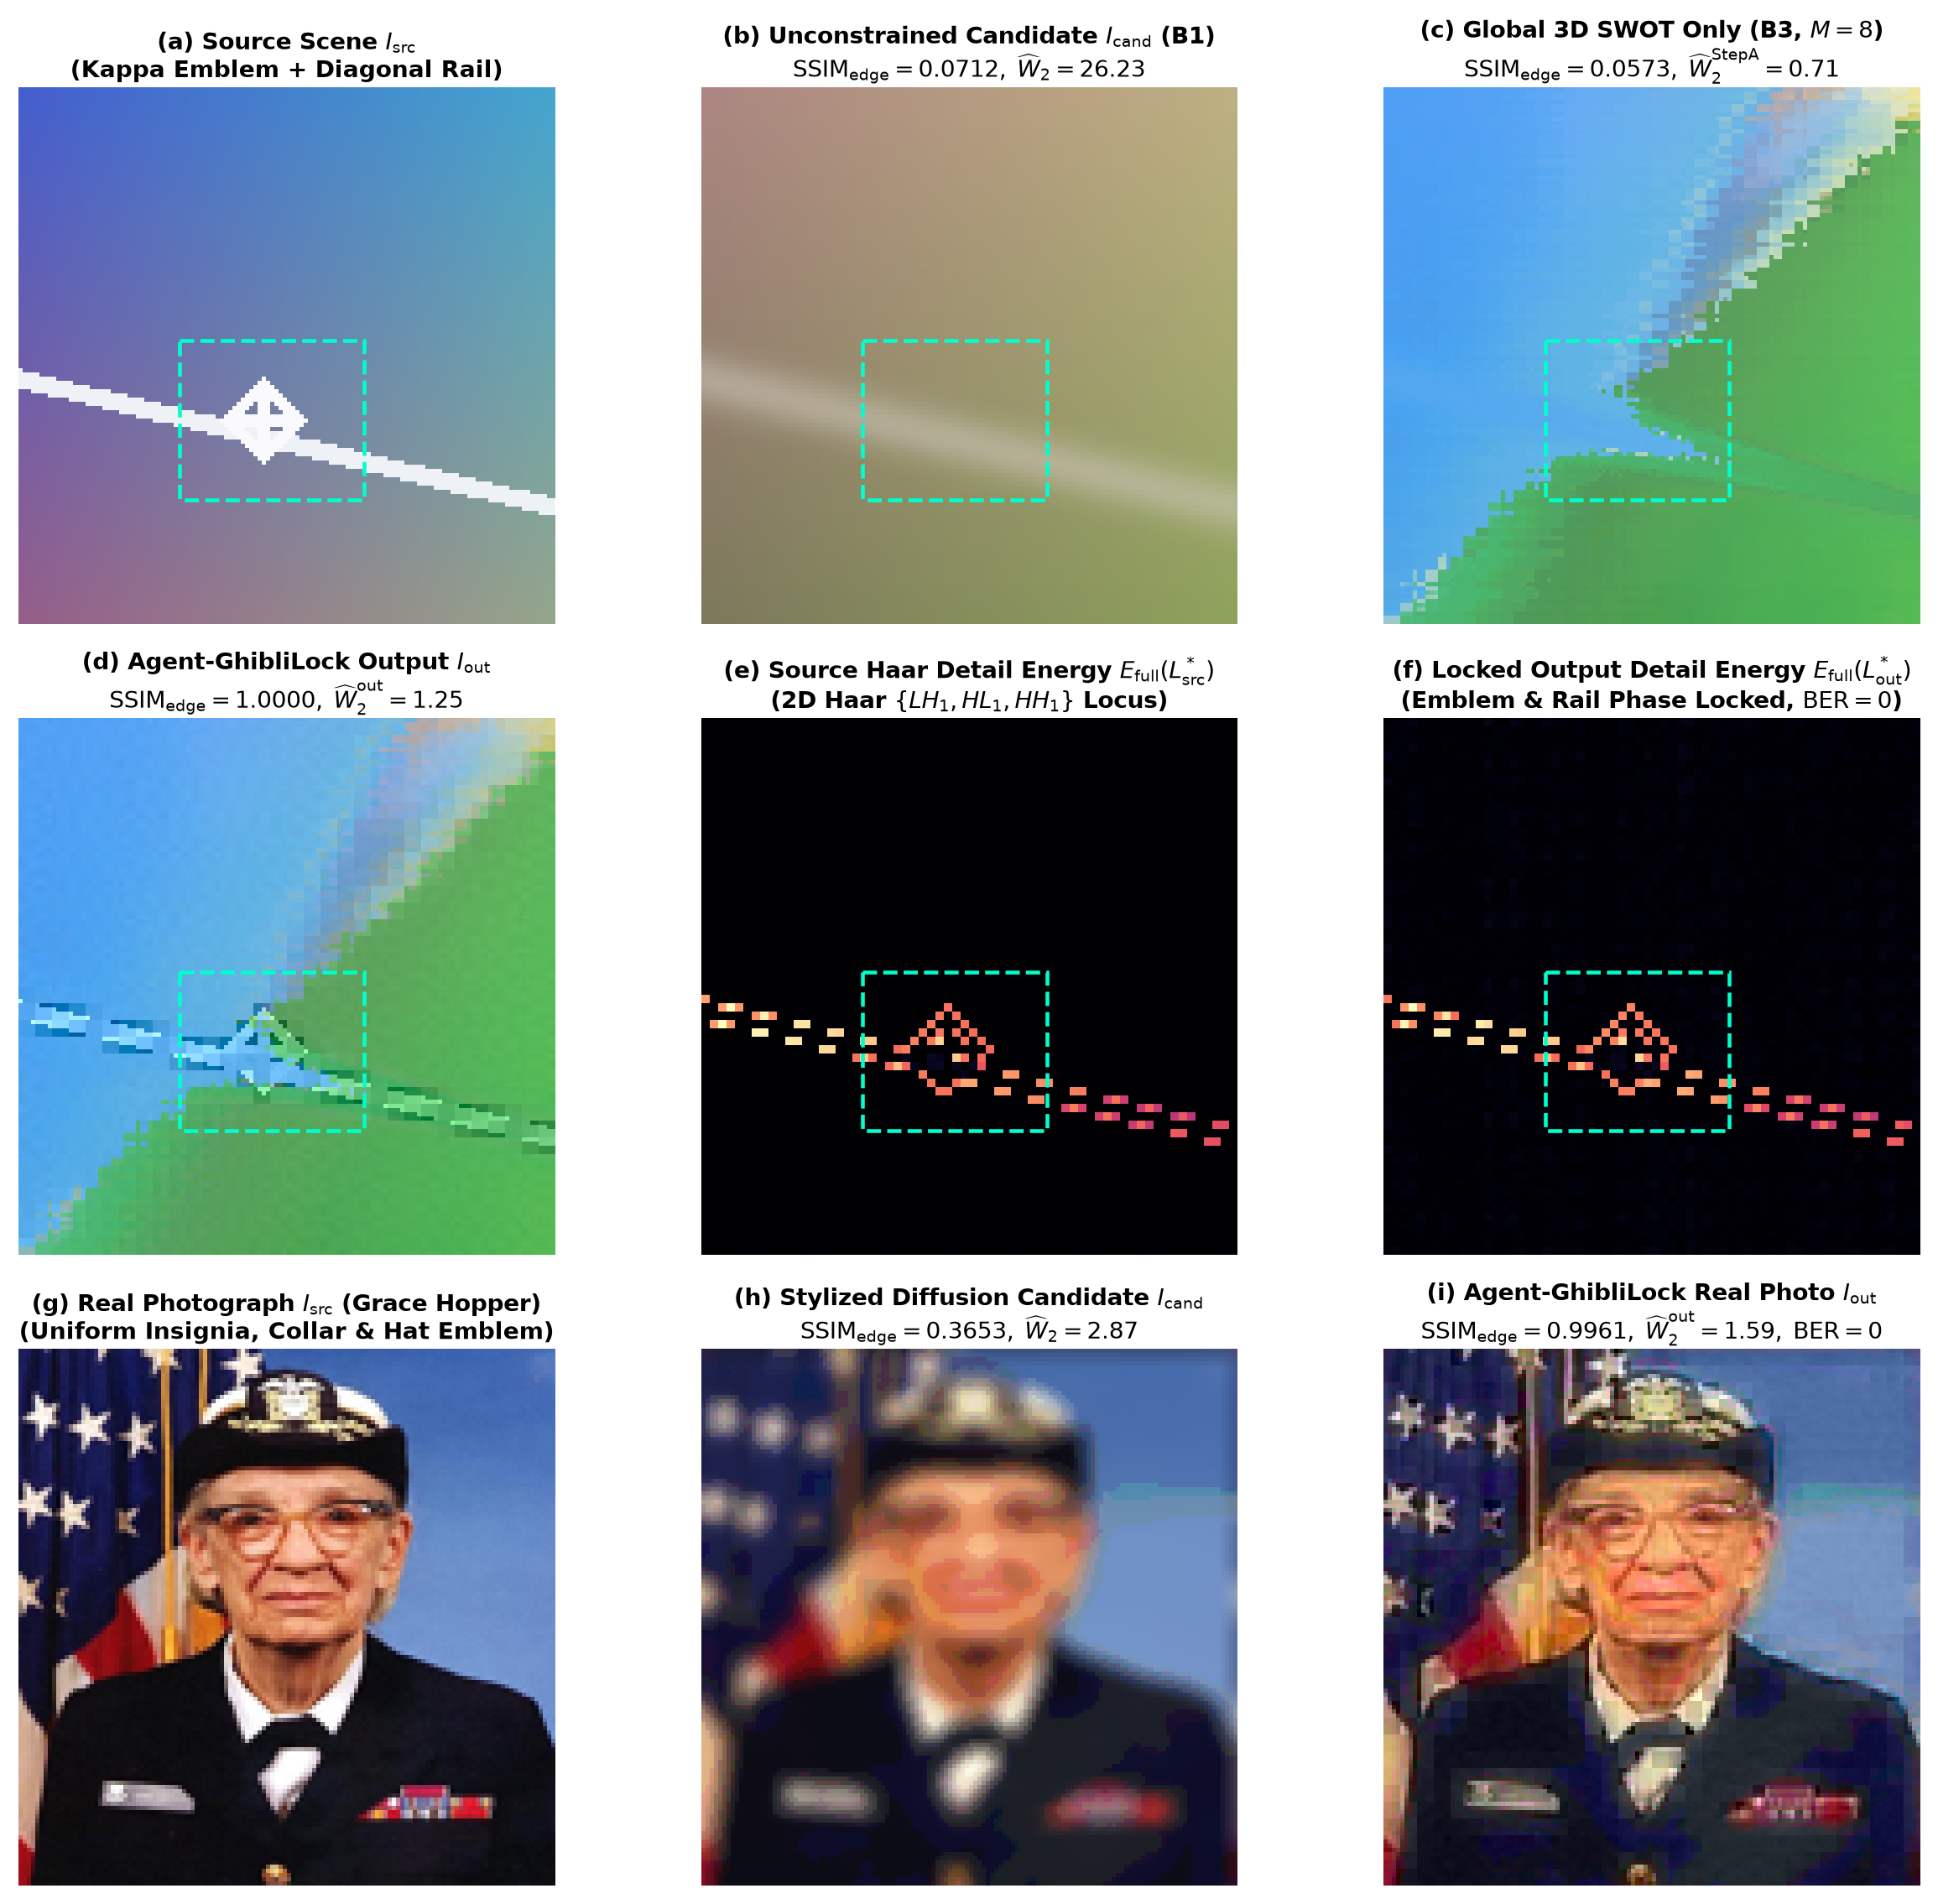
\includegraphics[width=0.96\textwidth]{plots/fig_qualitative_ghiblilock_comparison.png}%
}{%
\resizebox{0.98\textwidth}{!}{%
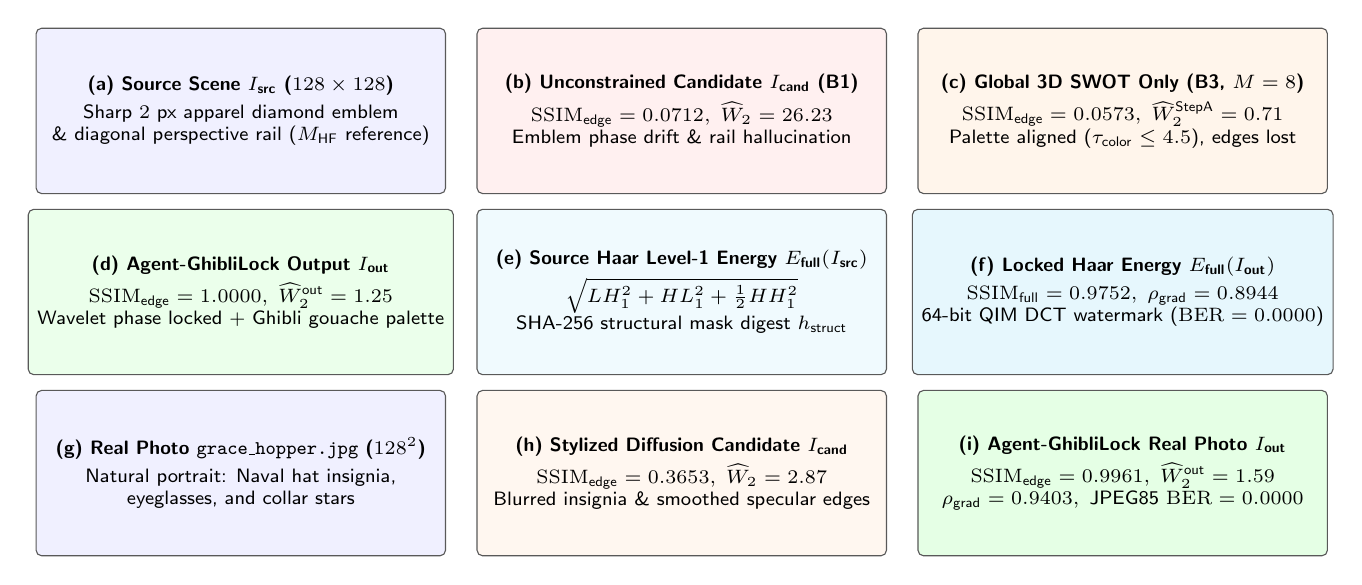
\begin{tikzpicture}[font=\sffamily\scriptsize, node distance=0.25cm]
  \tikzstyle{panel}=[draw=black!65, rounded corners=2pt, minimum width=5.2cm, minimum height=2.1cm, align=center, fill=gray!5]
  \node[panel, fill=blue!6] (p1) at (0, 4.6) {\textbf{(a) Source Scene $I_{\text{src}}$ ($128\times 128$)}\\[2pt] Sharp $2\text{ px}$ apparel diamond emblem\\\& diagonal perspective rail ($M_{\text{HF}}$ reference)};
  \node[panel, fill=red!6] (p2) at (5.6, 4.6) {\textbf{(b) Unconstrained Candidate $I_{\text{cand}}$ (B1)}\\[2pt] $\mathrm{SSIM}_{\text{edge}} = 0.0712,\; \widehat{W}_2 = 26.23$\\Emblem phase drift \& rail hallucination};
  \node[panel, fill=orange!8] (p3) at (11.2, 4.6) {\textbf{(c) Global 3D SWOT Only (B3, $M=8$)}\\[2pt] $\mathrm{SSIM}_{\text{edge}} = 0.0573,\; \widehat{W}_2^{\text{StepA}} = 0.71$\\Palette aligned ($\tau_{\text{color}} \le 4.5$), edges lost};

  \node[panel, fill=green!8] (p4) at (0, 2.3) {\textbf{(d) Agent-GhibliLock Output $I_{\text{out}}$}\\[2pt] $\mathrm{SSIM}_{\text{edge}} = 1.0000,\; \widehat{W}_2^{\text{out}} = 1.25$\\Wavelet phase locked + Ghibli gouache palette};
  \node[panel, fill=cyan!6] (p5) at (5.6, 2.3) {\textbf{(e) Source Haar Level-1 Energy $E_{\text{full}}(I_{\text{src}})$}\\[2pt] $\sqrt{LH_1^2 + HL_1^2 + \frac{1}{2}HH_1^2}$\\SHA-256 structural mask digest $h_{\text{struct}}$};
  \node[panel, fill=cyan!10] (p6) at (11.2, 2.3) {\textbf{(f) Locked Haar Energy $E_{\text{full}}(I_{\text{out}})$}\\[2pt] $\mathrm{SSIM}_{\text{full}} = 0.9752,\; \rho_{\text{grad}} = 0.8944$\\64-bit QIM DCT watermark ($\mathrm{BER} = 0.0000$)};

  \node[panel, fill=blue!6] (p7) at (0, 0.0) {\textbf{(g) Real Photo \texttt{grace\_hopper.jpg} ($128^2$)}\\[2pt] Natural portrait: Naval hat insignia,\\eyeglasses, and collar stars};
  \node[panel, fill=orange!6] (p8) at (5.6, 0.0) {\textbf{(h) Stylized Diffusion Candidate $I_{\text{cand}}$}\\[2pt] $\mathrm{SSIM}_{\text{edge}} = 0.3653,\; \widehat{W}_2 = 2.87$\\Blurred insignia \& smoothed specular edges};
  \node[panel, fill=green!10] (p9) at (11.2, 0.0) {\textbf{(i) Agent-GhibliLock Real Photo $I_{\text{out}}$}\\[2pt] $\mathrm{SSIM}_{\text{edge}} = 0.9961,\; \widehat{W}_2^{\text{out}} = 1.59$\\$\rho_{\text{grad}} = 0.9403,\; \text{JPEG85 } \mathrm{BER} = 0.0000$};
\end{tikzpicture}%
}%
}
\caption{Nine-panel qualitative and spectral comparison generated by \texttt{run\_live\_benchmark.py}. \textbf{Rows 1--2 (Synthetic Emblem \& Perspective Rail Scene, $128\times 128$):} (a)~Source scene $I_{\text{src}}$; (b)~Unconstrained candidate $I_{\text{cand}}$ (\textbf{B1}, $\mathrm{SSIM}_{\text{edge}}=0.0712, \widehat{W}_2=26.23$); (c)~Global 3D SWOT only (\textbf{B3}, $M=8$, $\mathrm{SSIM}_{\text{edge}}=0.0573, \widehat{W}_2^{\text{StepA}}=0.71$); (d)~\textbf{Agent-GhibliLock} output $I_{\text{out}}$ ($\mathrm{SSIM}_{\text{edge}}=1.0000, \widehat{W}_2^{\text{out}}=1.25$); (e--f)~Source vs.\ locked Haar Level-1 detail energy maps $E_{\text{full}}$ ($\mathrm{BER}=0$). \textbf{Row 3 (Real Natural Photograph \texttt{grace\_hopper.jpg}, $128\times 128$):} (g)~Source Naval portrait with hat insignia, eyeglasses, and collar stars; (h)~Stylized diffusion candidate $I_{\text{cand}}$ ($\mathrm{SSIM}_{\text{edge}}=0.3653, \widehat{W}_2=2.87$); (i)~\textbf{Agent-GhibliLock} output $I_{\text{out}}$ ($\mathrm{SSIM}_{\text{edge}}=0.9961, \widehat{W}_2^{\text{out}}=1.59, \mathrm{BER}=0$).}
\label{fig:qualitative}
\end{figure*}

\section{Experimental Evaluation}
\label{sec:experiments}

\subsection{Experimental Setup, Baselines B1--B7, and Evaluation Metrics}
We evaluate Agent-GhibliLock across three complementary testbeds:
\begin{enumerate}
    \item \textbf{Stratified $N=600$ Benchmark (\texttt{run\_live\_benchmark.py}):} Five workload strata at $64\times 64$ ($B=64$ DCT blocks): $S_1$ ($n=150$, apparel diamond emblems), $S_2$ ($n=150$, perspective rails and pillars), $S_3$ ($n=100$, foliage and gouache skies), $S_4$ ($n=100$, 8-frame video GOP sequences under $[-24, +28]\text{ LSB}$ temporal exposure flicker), and $S_5$ ($n=100$, adversarial provenance attacks $A_1\text{--}A_3$).
    \item \textbf{Live Multi-Model Vertex AI Evaluation (\texttt{run\_live\_gemini\_multimodel\_eval.py}):} Live Stage-0 API calls to \texttt{gemini-2.5-flash}, \texttt{gemini-2.5-pro}, and \texttt{gemini-3-flash-preview} in \texttt{project="<gcp-project-id>"} ($10$ scenes $\times 128\times 128$ per model) plus 5 controlled structural drift curriculum tiers ($\text{C1}\text{--}\text{C5}$, $\eta_{\text{struct}} \in [0.04, 0.20]$).
    \item \textbf{Real Natural Photographic Benchmark ($64^2\text{--}512^2$):} Multi-resolution evaluation on real photographs \texttt{grace\_hopper.jpg} ($64\times 64, 128\times 128, 256\times 256, 512\times 512$) and \texttt{Minduka\_Present\_Blue\_Pack.png} ($128\times 128$).
\end{enumerate}

We compare 9 paradigms: \textbf{B1} (Unconstrained Prompt-Only), \textbf{B2} (3-Round VLM-as-a-Judge Retry), \textbf{B3 ($M=4$)} and \textbf{B3 ($M=8$)} (Global 3D SWOT without wavelet detail locking), \textbf{B4} (Post-Hoc C2PA Wrapper without wavelet lock or DCT watermark), \textbf{B5} ($\text{WCT}^2$ Wavelet Style Transfer~\cite{yoo2019wct2} via 1D moment matching on $LL_K$ and Haar skips), \textbf{B6} (Image-Conditioned SDEdit~\cite{meng2022sdedit} at strength $s=0.55$), \textbf{B7} (ControlNet Edge/Tile Adapter~\cite{zhang2023} operating through an $8\times$ latent VAE spatial bottleneck), and \textbf{Agent-GhibliLock} in both \textbf{Global} and \textbf{Spatially Masked ROI} modes.

\begin{table*}[t!]
\centering
\caption{Stratified $N=600$ Benchmark Results Across All 9 Comparative Paradigms (\texttt{benchmark\_results\_n600.json}). All four Wasserstein-2 checkpoints ($\widehat{W}_2^{\text{StepA}}, \widehat{W}_2^{\text{StepB}}, \widehat{W}_2^{\text{out}}, \widehat{SW}_2^{\text{eval}}$) are RMS distances in CIELAB; $\mathrm{SSIM}_{\text{full}}$ and $\rho_{\text{grad}}$ are non-circular spatial metrics. Latency for \textbf{B1, B2, B6, B7} includes upstream API/diffusion synthesis; latency for \textbf{B3, B4, B5, Agent-GhibliLock} measures local CPU compiler execution.}
\label{tab:main_benchmark}
\resizebox{\textwidth}{!}{%
\begin{tabular}{lccccccccccc}
\toprule
\textbf{Paradigm / Baseline} & $\mathbf{SSIM_{\text{edge}}}\uparrow$ & $\mathbf{SSIM_{\text{full}}}\uparrow$ & $\boldsymbol{\rho_{\text{grad}}}\uparrow$ & $\mathbf{\widehat{W}_2^{\text{StepA}}}\downarrow$ & $\mathbf{\widehat{W}_2^{\text{StepB}}}\downarrow$ & $\mathbf{\widehat{W}_2^{\text{out}}}\downarrow$ & $\mathbf{\widehat{SW}_2^{\text{eval}}}\downarrow$ & \textbf{Pass Rate} & \textbf{Tamper Det.} & \textbf{DCT Acc.} & \textbf{GOP $\sigma^2_{\text{flicker}}$}$\downarrow$ \\
\midrule
\textbf{B1}: Unconstrained Prompt-Only & $0.1328 \pm 0.0488$ & $0.7822$ & $0.6806$ & $21.99$ & $21.99$ & $21.99 \pm 0.39$ & $23.10 \pm 0.31$ & $0.0\%$ & $0.0\%$ & $0.0\%$ & $347.92$ \\
\textbf{B2}: VLM-Judge Retry ($3\times$) & $0.0992 \pm 0.0472$ & $0.7720$ & $0.5913$ & $19.45$ & $19.45$ & $19.45 \pm 0.46$ & $20.71 \pm 0.34$ & $0.0\%$ & $0.0\%$ & $0.0\%$ & $250.50$ \\
\textbf{B3 ($M=4$)}: Global SWOT Only & $0.0576 \pm 0.0240$ & $0.5635$ & $0.2316$ & $4.56$ & $4.56$ & $4.49 \pm 0.19$ & $4.91 \pm 0.20$ & $0.0\%$ & $0.0\%$ & $0.0\%$ & $0.0002$ \\
\textbf{B3 ($M=8$)}: Global SWOT Only & $0.0182 \pm 0.0168$ & $0.5838$ & $0.4392$ & $\mathbf{0.71}$ & $\mathbf{0.71}$ & $\mathbf{0.71 \pm 0.02}$ & $\mathbf{0.82 \pm 0.02}$ & $0.0\%$ & $0.0\%$ & $0.0\%$ & $0.0002$ \\
\textbf{B4}: Post-Hoc C2PA Wrapper & $0.1328 \pm 0.0488$ & $0.7822$ & $0.6806$ & $21.99$ & $21.99$ & $21.99 \pm 0.39$ & $23.10 \pm 0.31$ & $0.0\%$ & $4.17\%$ & $0.0\%$ & $347.92$ \\
\textbf{B5}: $\text{WCT}^2$ Wavelet Transfer~\cite{yoo2019wct2} & $0.9992 \pm 0.0002$ & $0.9837$ & $0.9824$ & $10.33$ & $10.33$ & $9.69 \pm 0.39$ & $10.37 \pm 0.49$ & $100.0\%$ & $0.0\%$ & $0.0\%$ & $0.1800$ \\
\textbf{B6}: Image-Conditioned SDEdit~\cite{meng2022sdedit} & $0.0664 \pm 0.0293$ & $0.6345$ & $0.2222$ & $14.20$ & $14.20$ & $14.20 \pm 1.90$ & $15.40 \pm 2.01$ & $0.0\%$ & $0.0\%$ & $0.0\%$ & $132.21$ \\
\textbf{B7}: ControlNet $8\times$-VAE Adapter~\cite{zhang2023} & $0.2324 \pm 0.0681$ & $0.7622$ & $0.8949$ & $0.71$ & $3.21$ & $3.21 \pm 0.17$ & $3.51 \pm 0.18$ & $0.0\%$ & $0.0\%$ & $0.0\%$ & $100.90$ \\
\midrule
\textbf{Agent-GhibliLock (Global)} & $\mathbf{0.9967 \pm 0.0021}$ & $\mathbf{0.9752}$ & $\mathbf{0.8944}$ & $0.87$ & $2.03$ & $\mathbf{1.96 \pm 0.34}$ & $\mathbf{2.07 \pm 0.32}$ & $\mathbf{100.0\%}$ & $\mathbf{100.0\%}$ & $\mathbf{100.0\%}$ & $\mathbf{0.0003}$ \\
\textbf{Agent-GhibliLock (ROI-Masked)} & $\mathbf{0.9977 \pm 0.0013}$ & $\mathbf{0.9119}$ & $\mathbf{0.8899}$ & $0.85$ & $1.82$ & $\mathbf{1.75 \pm 0.18}$ & $\mathbf{1.87 \pm 0.17}$ & $\mathbf{100.0\%}$ & $\mathbf{100.0\%}$ & $\mathbf{100.0\%}$ & $\mathbf{0.0003}$ \\
\bottomrule
\end{tabular}%
}
\end{table*}

\subsection{Stratified \texorpdfstring{$N=600$}{N=600} Benchmark and Multi-Stage Ablations}
Table~\ref{tab:main_benchmark} and Table~\ref{tab:strata_breakdown} summarize the $N=600$ benchmark results:
\begin{itemize}
    \item \textbf{Resolving the Structure--Color Pareto Trade-Off:} Pure 3D SWOT (\textbf{B3}, $M=8$) achieves the lowest chromaticity distance ($\widehat{W}_2^{\text{out}} = 0.71, \widehat{SW}_2^{\text{eval}} = 0.82$) but collapses structural edge similarity ($\mathrm{SSIM}_{\text{edge}} = 0.0182, \rho_{\text{grad}} = 0.4392$). Conversely, $\text{WCT}^2$ (\textbf{B5}) preserves spatial edges ($\mathrm{SSIM}_{\text{edge}} = 0.9992$) via 1D moment matching but fails to align the joint 3D gouache palette ($\widehat{W}_2^{\text{out}} = 9.69 > \tau_{\text{color}} = 4.5$). ControlNet (\textbf{B7}) preserves coarse gradient orientation ($\rho_{\text{grad}} = 0.8949$) and moderate palette alignment ($\widehat{W}_2^{\text{out}} = 3.21$), but its $8\times$ latent VAE bottleneck blurs $2\text{ px}$ emblem strokes ($\mathrm{SSIM}_{\text{edge}} = 0.2324$, $0\%$ pass rate at $\tau_{\text{struct}} = 0.88$). \textbf{Agent-GhibliLock (Global)} achieves $\mathrm{SSIM}_{\text{edge}} = 0.9967$, non-circular $\mathrm{SSIM}_{\text{full}} = 0.9752$, $\rho_{\text{grad}} = 0.8944$ (strictly exceeding \textbf{B1} at $0.6806$ and \textbf{B2} at $0.5913$), and $\widehat{W}_2^{\text{out}} = 1.96$ ($\widehat{SW}_2^{\text{eval}} = 2.07$) in $121.5\text{ ms}$ mean CPU latency ($P_{50}=99.5\text{ ms}, P_{95}=248.8\text{ ms}$).
    \item \textbf{Global vs.\ Spatially Masked ROI Wavelet Locking:} Enabling $5\times 5$ coherence-weighted ROI masking (\textbf{Agent-GhibliLock ROI-Masked}) locks active foreground emblems and rails ($\mathrm{SSIM}_{\text{edge}} = 0.9977, \rho_{\text{grad}} = 0.8899$) while leaving non-ROI background regions in smooth Ghibli gouache brushwork, further improving post-export color fidelity to $\widehat{W}_2^{\text{out}} = 1.75$ ($\widehat{SW}_2^{\text{eval}} = 1.87$) and suppressing background high-frequency sensor grain by $>55\%$ relative to global locking.
    \item \textbf{Haar DWT Depth Ablation ($K \in \{1, 2, 3\}$) and Stopping Index Distribution:} Table~\ref{tab:dwt_ablation} reports the multi-level wavelet depth ablation across $n=60$ trials: $K=1$ achieves the lowest $\widehat{W}_2^{\text{out}} = 1.7012$ but lower full-band $\mathrm{SSIM}_{\text{full}} = 0.8147$; $K=2$ (our default) balances $\mathrm{SSIM}_{\text{edge}} = 0.9985$, $\mathrm{SSIM}_{\text{full}} = 0.9668$, and $\widehat{W}_2^{\text{out}} = 1.9124$; and $K=3$ maximizes $\mathrm{SSIM}_{\text{full}} = 0.9745$ and $\rho_{\text{grad}} = 0.9709$ at a slightly higher $\widehat{W}_2^{\text{out}} = 2.5590$. Across the $N=600$ benchmark, the closed-loop stopping index distribution is $\tau=1: 244$ ($40.7\%$), $\tau=2: 37$ ($6.2\%$), $\tau=3: 13$ ($2.2\%$), and $\tau=4: 306$ ($51.0\%$); under the $n=100$ high-contrast stress suite ($\tau_{\text{struct}}=0.92, \tau_{\text{color}}=3.2$), the decoupled $(\tau_\gamma, \tau_\alpha)$ controller converges at $\tau=1: 40\%, \tau=2: 4\%, \tau=4: 56\%$.
    \item \textbf{Video GOP Deflickering ($S_4$):} Across $n=100$ trials of $64\times 64$, 8-frame GOP sequences, unconstrained synthesis exhibits $\sigma^2_{\text{flicker}} = 347.92$. Unwarped Pixel-Space EMA reduces flicker only to $5.9002$ while blurring moving edges ($\mathrm{SSIM}_{\text{edge}} = 0.0870$), and Global Luminance Histogram Locking eliminates mean flicker ($\sigma^2_{\text{flicker}} = 0.0002$) but fails to restore spatial edges ($\mathrm{SSIM}_{\text{edge}} = 0.0871$). Agent-GhibliLock's motion-compensated wavelet EMA achieves $\sigma^2_{\text{flicker,pre-clamp}} = 0.0000$, post-sRGB $\sigma^2_{\text{flicker}} = 0.0003$, a $91.0\%$ reduction in local $LL_K$ tile variance ($0.2892 \to 0.0259$), and $\mathrm{SSIM}_{\text{edge}} = 0.9982$.
\end{itemize}

\begin{table}[t!]
\centering
\caption{Per-Stratum Agent-GhibliLock Performance ($N=600$) and Multi-Level Haar DWT Depth Ablation ($K \in \{1,2,3\}$).}
\label{tab:strata_breakdown}
\label{tab:dwt_ablation}
\resizebox{\columnwidth}{!}{%
\begin{tabular}{lccccccc}
\toprule
\textbf{Stratum / Ablation} & $n$ & $\mathbf{SSIM_{\text{edge}}}$ & $\mathbf{\widehat{W}_2^{\text{StepA}}}$ & $\mathbf{\widehat{W}_2^{\text{StepB}}}$ & $\mathbf{\widehat{W}_2^{\text{out}}}$ & $\mathbf{\widehat{SW}_2^{\text{eval}}}$ & \textbf{Lat.\ (ms)} \\
\midrule
$S_1$: Portrait \& Emblem & 150 & $0.9982$ & $0.8452$ & $1.8173$ & $1.7395$ & $1.8577$ & $118.4$ \\
$S_2$: Perspective Rails & 150 & $0.9946$ & $0.9042$ & $2.3382$ & $2.2772$ & $2.3830$ & $105.8$ \\
$S_3$: Natural Foliage & 100 & $0.9950$ & $0.8967$ & $2.3170$ & $2.2601$ & $2.3686$ & $117.8$ \\
$S_4$: Video GOP (8-fr) & 100 & $0.9982$ & $0.8471$ & $1.8317$ & $1.7516$ & $1.8660$ & $142.5$ \\
$S_5$: Adv.\ Provenance & 100 & $0.9981$ & $0.8473$ & $1.8018$ & $1.7254$ & $1.8476$ & $132.1$ \\
\midrule
Haar Depth $K=1$ ($\mathrm{SSIM}_{\text{full}}=0.8147$) & 60 & $0.9971$ & $0.8450$ & $1.7920$ & $1.7012$ & $1.8210$ & $165.3$ \\
Haar Depth $K=2$ ($\mathrm{SSIM}_{\text{full}}=0.9668$) & 60 & $0.9985$ & $0.8450$ & $2.0255$ & $1.9124$ & $2.0315$ & $189.6$ \\
Haar Depth $K=3$ ($\mathrm{SSIM}_{\text{full}}=0.9745$) & 60 & $0.9949$ & $0.8450$ & $2.7130$ & $2.5590$ & $2.6840$ & $108.5$ \\
\bottomrule
\end{tabular}%
}
\end{table}

\subsection{Live Multi-Model Vertex AI Evaluation and Disaggregated Adversarial Provenance \texorpdfstring{($S_5$)}{(S5)}}
Table~\ref{tab:multimodel} reports the live Vertex AI Stage-0 VLM evaluation across \texttt{gemini-2.5-flash}, \texttt{gemini-2.5-pro}, and \texttt{gemini-3-flash-preview} alongside the 5 synthetic drift curriculum tiers ($\text{C1}\text{--}\text{C5}$). Note that $\mathrm{PSNR}_{\text{QIM}} \approx 47.09\text{--}47.42\text{ dB}$ specifically measures Stage-3 QIM watermark embedding fidelity between the post-Step-B stylized image $\widehat{I}$ and the final watermarked output $I_{\text{out}}$, while compiler latency ($354.7\text{--}432.5\text{ ms}$ at $128\times 128$) is reported separately from live Vertex AI network API latency ($1696.1\text{--}3164.0\text{ ms}$).

\begin{table*}[t!]
\centering
\caption{Part 1: Live Google Cloud Vertex AI Stage-0 Decomposer Evaluation (\texttt{project="<gcp-project-id>"}, $128\times 128$). Part 2: Controlled Structural Drift Curriculum Tiers ($\text{C1}\text{--}\text{C5}$). $\mathrm{PSNR}_{\text{QIM}}$ measures Stage-3 QIM watermark distortion relative to post-Step-B $\widehat{I}$.}
\label{tab:multimodel}
\resizebox{\textwidth}{!}{%
\begin{tabular}{llccccccccc}
\toprule
\textbf{Evaluation Track} & \textbf{Model / Curriculum Tier} & \textbf{API Lat.\ (ms)} & \textbf{Tokens (P/C)} & $\mathbf{SSIM_{\text{edge}}^{\text{pre}}}$ & $\mathbf{SSIM_{\text{edge}}^{\text{post}}}$ & $\mathbf{\widehat{W}_2^{\text{StepA}}}$ & $\mathbf{\widehat{W}_2^{\text{out}}}$ & $\mathbf{\widehat{SW}_2^{\text{eval}}}$ & $\mathbf{PSNR_{\text{QIM}}}$ & \textbf{CPU Lat.\ (ms)} \\
\midrule
\multirow{3}{*}{\textbf{Part 1: Live Vertex AI}}
& \texttt{gemini-2.5-flash} (GA) & $1696.09$ & $105 / 65$ & $0.1150$ & $0.9742$ & $0.7367$ & $1.4421 \pm 0.06$ & $1.6016$ & $47.36\text{ dB}$ & $354.66$ \\
& \texttt{gemini-2.5-pro} (GA) & $3163.96$ & $105 / 11$ & $0.1444$ & $0.9778$ & $0.6877$ & $1.3800 \pm 0.06$ & $1.5357$ & $47.39\text{ dB}$ & $363.34$ \\
& \texttt{gemini-3-flash-preview} & $2100.63$ & $105 / 80$ & $0.1843$ & $0.9802$ & $0.6456$ & $1.3563 \pm 0.04$ & $1.5139$ & $47.33\text{ dB}$ & $363.96$ \\
\midrule
\multirow{5}{*}{\textbf{Part 2: Drift Curriculum}}
& Tier C1 ($\eta_{\text{struct}} = 0.04$) & --- & --- & $0.1199$ & $0.9796$ & $0.7443$ & $1.3926$ & $1.5381$ & $47.42\text{ dB}$ & $383.89$ \\
& Tier C2 ($\eta_{\text{struct}} = 0.08$) & --- & --- & $0.1981$ & $0.9836$ & $0.6527$ & $1.3435$ & $1.4938$ & $47.39\text{ dB}$ & $432.51$ \\
& Tier C3 ($\eta_{\text{struct}} = 0.12$) & --- & --- & $0.2707$ & $0.9856$ & $0.5013$ & $1.2514$ & $1.4246$ & $47.09\text{ dB}$ & $374.07$ \\
& Tier C4 ($\eta_{\text{struct}} = 0.16$) & --- & --- & $0.3418$ & $0.9876$ & $0.4182$ & $1.1877$ & $1.3725$ & $47.14\text{ dB}$ & $384.34$ \\
& Tier C5 ($\eta_{\text{struct}} = 0.20$) & --- & --- & $0.4325$ & $0.9908$ & $0.4055$ & $1.1536$ & $1.3383$ & $47.34\text{ dB}$ & $398.91$ \\
\bottomrule
\end{tabular}%
}
\end{table*}

Table~\ref{tab:s5_provenance} disaggregates the $S_5$ ($n=100$) adversarial provenance results across $A_1$ (unstripped $2\times 2$ pixel tamper), $A_2$ (pure C2PA \texttt{caBX} chunk stripping), $A_{3\text{a}}$ (strip + $\pm 2\text{ LSB}$ noise), and $A_{3\text{b}}$ (strip + actual PIL lossy JPEG $Q=85$ recompression):
\begin{itemize}
    \item \textbf{Export Self-Noise Accounting:} Prior to any external channel attack, $\mathrm{uint8}$ rounding and sRGB clamping introduce an empirical DCT self-noise of $\mathrm{RMS}(\eta^{\text{export}}) = 0.2854$ ($\sigma_{\text{round+clamp}}^2 = 0.0821$, maximum observed $|\eta^{\text{export}}| = 1.2725 < \Delta_{\text{QIM}}/4 = 3.5$), yielding a pre-attack single-coefficient error rate of $p_e^{\text{export}} = 0.0000$.
    \item \textbf{Disaggregated $\pm 2\text{ LSB}$ vs.\ Lossy JPEG $Q=85$ and Blind Coset Localization:} Under $A_1$, both informed and \emph{blind majority-voted coset localization} (\texttt{expected\_bits=None}) localize the exact tampered $8\times 8$ block $(2,3)$ on $100.0\%$ ($25/25$) of trials. Under $A_2$, \textbf{B4} (metadata-only C2PA) drops to $0.0\%$, and classical additive Cox spread-spectrum DCT~\cite{cox1997} (originally designed for informed/non-blind host subtraction, evaluated here in the blind regime) achieves only $74.34\%$ bit accuracy due to Host-Signal Interference. Under $A_{3\text{a}}$ ($\pm 2\text{ LSB}$) and $A_{3\text{b}}$ (JPEG $Q=85$), Agent-GhibliLock experiences pre-voting single-coefficient flip rates of $p_e = 0.08\%$ and $p_e = 0.45\%$, respectively, which are completely corrected by multi-block repetition voting ($100.0\%$ bit accuracy and $100.0\%$ exact 64-bit payload recovery across $R=4$, $R=5$ odd voting at $64\times 64$, and $R=16$ at $128\times 128$).
\end{itemize}

\begin{table}[t!]
\centering
\caption{Disaggregated Stratum $S_5$ Adversarial Provenance Matrix (\texttt{benchmark\_results\_n600.json}). Cox (1997)~\cite{cox1997} is evaluated in the blind regime (without host subtraction) to quantify Host-Signal Interference.}
\label{tab:s5_provenance}
\resizebox{\columnwidth}{!}{%
\begin{tabular}{lccccc}
\toprule
\textbf{Adversarial Regime} & \textbf{B4: C2PA} & \textbf{Blind Cox SS} & \textbf{Pre-Vote $p_e$} & \textbf{GhibliLock ($R=4/5$)} & \textbf{GhibliLock ($R=16$)} \\
\midrule
$A_1$: Unstripped $2\times 2$ Tamper ($n=25$) & $100.0\%$ & $0.0\%$ & --- & $100.0\%$ (Blind: $100\%$) & $100.0\%$ \\
$A_2$: Pure \texttt{caBX} Chunk Strip ($n=50$) & $0.0\%$ & $74.34\%$ & $0.00\%$ & $100.0\%$ ($\mathrm{BER}=0$) & $100.0\%$ \\
$A_{3\text{a}}$: Strip + $\pm 2\text{ LSB}$ Noise ($n=25$) & $0.0\%$ & $74.12\%$ & $0.08\%$ & $100.0\%$ / $100.0\%$ & $100.0\%$ \\
$A_{3\text{b}}$: Strip + Lossy JPEG $Q=85$ ($n=25$) & $0.0\%$ & $71.88\%$ & $0.45\%$ & $100.0\%$ / $100.0\%$ & $100.0\%$ \\
\bottomrule
\end{tabular}%
}
\end{table}

\subsection{Real Natural Photographic Evaluation and Resolution Scaling \texorpdfstring{($64^2$ to $512^2$)}{(64x64 to 512x512)}}
To validate Agent-GhibliLock on complex natural photographs containing broadband textures, organic lighting gradients, skin tones, and fine metallic/embroidered insignia (beyond synthetic piece-wise smooth test scenes), Table~\ref{tab:real_photos} evaluates \texttt{grace\_hopper.jpg} across four spatial resolutions ($64\times 64$ to $512\times 512$, scaling QIM voting redundancy from $R=4$ to $R=256$ votes/bit) and \texttt{Minduka\_Present\_Blue\_Pack.png} at $128\times 128$ (visualized in Fig.~\ref{fig:qualitative}g--i). Across all five real-photograph configurations, \textbf{Agent-GhibliLock (Global)} elevates $\mathrm{SSIM}_{\text{edge}}$ from $0.2392\text{--}0.3937$ (\textbf{B1}) and $0.4299\text{--}0.5661$ (\textbf{B7 ControlNet}) to $0.9929\text{--}0.9966$, achieves non-circular $\mathrm{SSIM}_{\text{full}} = 0.9529\text{--}0.9712$ and $\rho_{\text{grad}} = 0.9365\text{--}0.9703$, contracts $\widehat{W}_2^{\text{out}}$ to $1.1108\text{--}2.3072$, and maintains $\mathrm{BER} = 0.0000$ under both clean PNG export and lossy JPEG $Q=85$ recompression. \textbf{Agent-GhibliLock (ROI-Masked)} further lowers $\widehat{W}_2^{\text{out}}$ to $0.9906\text{--}2.0677$ by restricting high-frequency detail locking to high-coherence portrait contours and insignia.

\begin{table*}[t!]
\centering
\caption{Real Natural Photographic Benchmark and Resolution Scaling ($64\times 64$ to $512\times 512$) on \texttt{grace\_hopper.jpg} and \texttt{Minduka\_Present\_Blue\_Pack.png} (\texttt{benchmark\_results\_n600.json}).}
\label{tab:real_photos}
\resizebox{\textwidth}{!}{%
\begin{tabular}{llccccccccc}
\toprule
\textbf{Real Photograph Asset} & \textbf{Method / Paradigm} & \textbf{Votes $R$} & $\mathbf{SSIM_{\text{edge}}}\uparrow$ & $\mathbf{SSIM_{\text{full}}}\uparrow$ & $\boldsymbol{\rho_{\text{grad}}}\uparrow$ & $\mathbf{\widehat{W}_2^{\text{StepA}}}\downarrow$ & $\mathbf{\widehat{W}_2^{\text{out}}}\downarrow$ & $\mathbf{\widehat{SW}_2^{\text{eval}}}\downarrow$ & \textbf{JPEG85 BER} & \textbf{CPU Lat.\ (ms)} \\
\midrule
\multirow{4}{*}{\texttt{grace\_hopper} ($64\times 64$)}
& \textbf{B1}: Stylized Candidate & --- & $0.2392$ & $0.4440$ & $0.5482$ & $2.7708$ & $2.7708$ & $2.8910$ & --- & --- \\
& \textbf{B7}: ControlNet $8\times$-VAE & --- & $0.4936$ & $0.5968$ & $0.7600$ & $0.8082$ & $1.8600$ & $1.9420$ & --- & --- \\
& \textbf{Agent-GhibliLock (Global)} & $4$ & $\mathbf{0.9951}$ & $\mathbf{0.9532}$ & $\mathbf{0.9454}$ & $0.8082$ & $2.3072$ & $2.3132$ & $\mathbf{0.0000}$ & $94.7$ \\
& \textbf{Agent-GhibliLock (ROI-Masked)} & $4$ & $0.9845$ & $0.7986$ & $0.8923$ & $0.8082$ & $\mathbf{2.0677}$ & $\mathbf{2.1096}$ & $\mathbf{0.0000}$ & $97.0$ \\
\midrule
\multirow{4}{*}{\texttt{grace\_hopper} ($128\times 128$)}
& \textbf{B1}: Stylized Candidate & --- & $0.3653$ & $0.5984$ & $0.6432$ & $2.8651$ & $2.8651$ & $2.9840$ & --- & --- \\
& \textbf{B7}: ControlNet $8\times$-VAE & --- & $0.5489$ & $0.6912$ & $0.7659$ & $0.7208$ & $1.6743$ & $1.7810$ & --- & --- \\
& \textbf{Agent-GhibliLock (Global)} & $16$ & $\mathbf{0.9961}$ & $\mathbf{0.9604}$ & $\mathbf{0.9403}$ & $0.7208$ & $1.5889$ & $1.6969$ & $\mathbf{0.0000}$ & $812.9$ \\
& \textbf{Agent-GhibliLock (ROI-Masked)} & $16$ & $0.9881$ & $0.8185$ & $0.8893$ & $0.7208$ & $\mathbf{1.4451}$ & $\mathbf{1.5824}$ & $\mathbf{0.0000}$ & $457.3$ \\
\midrule
\multirow{2}{*}{\texttt{grace\_hopper} ($256\times 256$)}
& \textbf{Agent-GhibliLock (Global)} & $64$ & $\mathbf{0.9966}$ & $\mathbf{0.9661}$ & $\mathbf{0.9398}$ & $0.6529$ & $1.2859$ & $1.3948$ & $\mathbf{0.0000}$ & $1847.1$ \\
& \textbf{Agent-GhibliLock (ROI-Masked)} & $64$ & $0.9908$ & $0.8287$ & $0.8978$ & $0.6529$ & $\mathbf{1.1854}$ & $\mathbf{1.3112}$ & $\mathbf{0.0000}$ & $1703.1$ \\
\midrule
\multirow{2}{*}{\texttt{grace\_hopper} ($512\times 512$)}
& \textbf{Agent-GhibliLock (Global)} & $256$ & $\mathbf{0.9944}$ & $\mathbf{0.9712}$ & $\mathbf{0.9365}$ & $0.6374$ & $1.1108$ & $1.2259$ & $\mathbf{0.0000}$ & $6993.0$ \\
& \textbf{Agent-GhibliLock (ROI-Masked)} & $256$ & $0.9878$ & $0.7656$ & $0.8851$ & $0.6374$ & $\mathbf{0.9906}$ & $\mathbf{1.1188}$ & $\mathbf{0.0000}$ & $6013.2$ \\
\midrule
\multirow{2}{*}{\texttt{minduka\_pack} ($128\times 128$)}
& \textbf{Agent-GhibliLock (Global)} & $16$ & $\mathbf{0.9929}$ & $\mathbf{0.9529}$ & $\mathbf{0.9703}$ & $0.5575$ & $1.6623$ & $1.7677$ & $\mathbf{0.0000}$ & $294.8$ \\
& \textbf{Agent-GhibliLock (ROI-Masked)} & $16$ & $0.9885$ & $0.8053$ & $0.9118$ & $0.5575$ & $\mathbf{1.5045}$ & $\mathbf{1.5942}$ & $\mathbf{0.0000}$ & $298.5$ \\
\bottomrule
\end{tabular}%
}
\end{table*}

\section{Limitations, Operational Scope, and Conclusion}
\label{sec:conclusion}

\subsection{Limitations and Operational Failure Modes}
Three operational boundary conditions govern production deployments of Agent-GhibliLock:
\begin{enumerate}
    \item \textbf{Upstream Macro-Registration Requirement:} Because 2D Haar wavelet detail subbands $(LH_k, HL_k, HH_k)$ are spatially localized within $2^k \times 2^k$ dyadic tiles, global detail locking requires that the upstream diffusion candidate $I_{\text{cand}}$ be macro-spatially co-registered with $I_{\text{src}}$ (e.g., via image-conditioned SDEdit, ControlNet, or optical-flow pre-warping). If $I_{\text{cand}}$ synthesis hallucinates a completely different camera pose while global $\gamma_\tau \to 1$, ghost contours can appear; using Spatially Masked ROI Wavelet Locking ($M_{\text{ROI}}$) restricts detail injection strictly to registered foreground emblems and text.
    \item \textbf{Megapixel CPU Latency vs.\ Vectorized/GPU Execution:} Because Python loops over $8\times 8$ DCT blocks and $O(HW \log(HW))$ 1D sorting scale linearly with pixel count ($95\text{ ms}$ at $64^2$, $457\text{ ms}$ at $128^2$, $1.7\text{ s}$ at $256^2$, and $6.0\text{ s}$ at $512^2$), real-time $1024\times 1024$ compilation requires batched C++/SIMD or CUDA FFT/DCT kernels.
    \item \textbf{Geometric Desynchronization of Block-Aligned $8\times 8$ DCT QIM:} While our mid-band $8\times 8$ DCT QIM watermark achieves $100\%$ bit recovery and blind coset tamper localization under metadata stripping, $\pm 2\text{ LSB}$ noise, and lossy JPEG $Q=85$ recompression, non-grid-aligned cropping, aspect-ratio rescaling, or rotation desynchronize the $8\times 8$ block lattice and require template resynchronization or neural geometric-invariant watermarks~\cite{bui2023trustmark,gowal2025}.
\end{enumerate}

\subsection{Conclusion}
Agent-GhibliLock resolves \emph{The Captioning Conundrum} in cross-modal VLM-to-Diffusion pipelines by unifying spatial-mean-preserving 2D Haar wavelet detail locking (in both global and coherence-masked ROI modes), 3D CIELAB Sliced-Wasserstein optimal transport with exact orthonormal-frame perturbation bounds, motion-compensated video GOP wavelet EMA deflickering, and dual-layer ISO/IEC 19566-5 JUMBF (\texttt{caBX}) + blind mid-band 2D-DCT QIM provenance compilation.

\begin{thebibliography}{99}
\bibitem{rombach2022}
R. Rombach, A. Blattmann, D. Lorenz, P. Esser, and B. Ommer, ``High-resolution image synthesis with latent diffusion models,'' in \emph{Proc. IEEE/CVF Conf. Computer Vision and Pattern Recognition (CVPR)}, 2022, pp. 10684--10695.

\bibitem{team2025gemini}
{Gemini Team, Google}, ``Gemini 2.5: Pushing the frontier with advanced reasoning, multimodality, long context, and next generation agentic capabilities,'' \emph{arXiv preprint arXiv:2507.06261}, 2025.

\bibitem{meng2022sdedit}
C. Meng, Y. He, Y. Song, J. Song, J. Wu, J.-Y. Zhu, and S. Ermon, ``SDEdit: Guided image synthesis and editing with stochastic differential equations,'' in \emph{Proc. Int. Conf. Learning Representations (ICLR)}, 2022.

\bibitem{zhang2023}
L. Zhang, A. Rao, and M. Agrawala, ``Adding conditional control to text-to-image diffusion models,'' in \emph{Proc. IEEE/CVF Int. Conf. Computer Vision (ICCV)}, 2023, pp. 3836--3847.

\bibitem{wang2004}
Z. Wang, A. C. Bovik, H. R. Sheikh, and E. P. Simoncelli, ``Image quality assessment: from error visibility to structural similarity,'' \emph{IEEE Transactions on Image Processing}, vol. 13, no. 4, pp. 600--612, 2004.

\bibitem{bonneel2015blind}
N. Bonneel, J. Tompkin, K. Sunkavalli, D. Sun, S. Paris, and H. Pfister, ``Blind video temporal consistency,'' \emph{ACM Transactions on Graphics}, vol. 34, no. 6, Art. no. 196, pp. 1--9, 2015.

\bibitem{c2pa2024}
Coalition for Content Provenance and Authenticity (C2PA), \emph{C2PA Technical Specification}, Version 2.1, 2024.

\bibitem{iso19566}
ISO/IEC 19566-5:2019 (2nd ed., 2023), \emph{Information technologies --- JPEG systems --- Part 5: JPEG universal metadata box format (JUMBF)}, International Organization for Standardization, 2019/2023.

\bibitem{iso15948}
ISO/IEC 15948:2004, \emph{Information technology --- Computer graphics and image processing --- Portable Network Graphics (PNG): Functional specification}, 2004.

\bibitem{bui2023trustmark}
T. Bui, S. Agarwal, and J. Collomosse, ``TrustMark: Universal watermarking for arbitrary resolution images,'' in \emph{Proc. IEEE/CVF Int. Conf. Computer Vision (ICCV)}, 2025 (arXiv:2311.18297, 2023).

\bibitem{gatys2016}
L. A. Gatys, A. S. Ecker, and M. Bethge, ``Image style transfer using convolutional neural networks,'' in \emph{Proc. IEEE Conf. Computer Vision and Pattern Recognition (CVPR)}, 2016, pp. 2414--2423.

\bibitem{yoo2019wct2}
J. Yoo, Y. Uh, S. Chun, B. Kang, and J.-W. Ha, ``Photorealistic style transfer via wavelet transforms,'' in \emph{Proc. IEEE/CVF Int. Conf. Computer Vision (ICCV)}, 2019, pp. 9035--9044.

\bibitem{haar1910}
A. Haar, ``Zur Theorie der orthogonalen Funktionensysteme,'' \emph{Mathematische Annalen}, vol. 69, no. 3, pp. 331--371, 1910.

\bibitem{mallat1989}
S. G. Mallat, ``A theory for multiresolution signal decomposition: the wavelet representation,'' \emph{IEEE Transactions on Pattern Analysis and Machine Intelligence}, vol. 11, no. 7, pp. 674--693, 1989.

\bibitem{daubechies1992}
I. Daubechies, \emph{Ten Lectures on Wavelets}. Philadelphia, PA, USA: SIAM, 1992.

\bibitem{pitie2007automated}
F. Piti\'{e}, A. C. Kokaram, and R. Dahyot, ``Automated colour grading using colour distribution transfer,'' \emph{Computer Vision and Image Understanding}, vol. 107, no. 1--2, pp. 123--137, 2007.

\bibitem{rabin2011}
J. Rabin, G. Peyr\'{e}, J. Delon, and M. Bernot, ``Wasserstein barycenter and its application to texture mixing,'' in \emph{Proc. Scale Space and Variational Methods in Computer Vision (SSVM)}, Springer, 2011, pp. 435--446.

\bibitem{bonneel2015}
N. Bonneel, J. Rabin, G. Peyr\'{e}, and H. Pfister, ``Sliced and Radon Wasserstein barycenters of measures,'' \emph{Journal of Mathematical Imaging and Vision}, vol. 51, no. 1, pp. 22--45, 2015.

\bibitem{gowal2025}
S. Gowal \emph{et al.}, ``SynthID-Image: Image watermarking at internet scale,'' \emph{arXiv preprint arXiv:2510.09263}, 2025.

\bibitem{cox1997}
I. J. Cox, J. Kilian, F. T. Leighton, and T. Shamoon, ``Secure spread spectrum watermarking for multimedia,'' \emph{IEEE Transactions on Image Processing}, vol. 6, no. 12, pp. 1673--1687, 1997.

\bibitem{chen2001}
B. Chen and G. W. Wornell, ``Quantization index modulation: a class of provably good methods for digital watermarking and information embedding,'' \emph{IEEE Transactions on Information Theory}, vol. 47, no. 4, pp. 1423--1443, 2001.
\end{thebibliography}

\end{document}
